\documentclass[UKenglish]{DUO/ifimaster}
\usepackage[utf8]{inputenc}           %% ... or latin1
\usepackage[T1]{fontenc,url}
\urlstyle{sf}
\usepackage{babel,textcomp,csquotes,DUO/duomasterforside,varioref,graphicx}
\usepackage[backend=biber,style=numeric-comp,sorting=none]{biblatex}
\usepackage{amsmath,amssymb,amsfonts}
\usepackage{algorithmic}
\usepackage{textcomp}
\usepackage{xcolor}
\usepackage{textgreek}
\usepackage{float}
\usepackage{graphicx}
\usepackage{titlesec}
\usepackage{glossaries-extra}
\usepackage{verbatim}

\raggedbottom %%reduces the gaps between the paragraphs
\addbibresource{bibliography.bib}            %% ... or whatever

\usepackage{glossaries-extra}
\setabbreviationstyle[acronym]{long-short}


\newacronym{cnn}{CNN}{Convolutional Neural Network}
\newacronym{rnn}{RNN}{Recurrent Neural Network}
\newacronym{cpu}{CPU}{Central Processing Unit}
\newacronym{gpu}{GPU}{Graphics Processing Unit}
\newacronym{vqa}{VQA}{Visual Question Answering}
\newacronym{xai}{XAI}{Explainable Artificial Intelligence} % Should it be Explainable or eXplainable?
\newacronym{ai}{AI}{Artificial Intelligence}
\newacronym{ml}{ML}{Machine Learning}
\newacronym{shap}{SHAP}{SHapley Additive exPlanations}
\newacronym{lime}{LIME}{Local Interpretable Model-agnostic Explanations}
\newacronym{knn}{k-NN}{k-Nearest Neighbors}
\newacronym{gradcam}{Grad-CAM}{Gradient-weighted Class Activation Mapping}
\newacronym{flex}{FLEX}{Faithful Linguistic Explanations}
\newacronym{lstm}{LSTM}{Long Short-Term Memory}
\newacronym{sota}{SOTA}{State-of-the-Art}
\newacronym{nlp}{NLP}{Natural Language Processing}
\newacronym{bvlc}{BVLC}{The Berkeley Vision and Learning Center} % Developed Caffe together with BAIR
\newacronym{bair}{BAIR}{Berkeley AI Research} % Developed Caffe together with BVLC
\newacronym{svm}{SVM}{Support Vector Machines}
\newacronym{svd}{SVD}{Singular Value Decomposition}
\newacronym{pca}{PCA}{Principal Component Analysis}
\newacronym{imagenet}{ILSVRC}{ImageNet Large Scale Visual Recognition Challenge}
\newacronym{ann}{ANN}{Artificial Neural Network}
\newacronym{vit}{ViT}{Vision Transformer}
\newacronym{bert}{BERT}{Bidirectional Encoder Representations from Transformers}
\newacronym{bart}{BART}{Bidirectional Auto-Regressive Transformers}
\newacronym{gpt}{GPT}{Generative Pre-trained Transformer}
\newacronym{vram}{VRAM}{Video RAM}
\newacronym{lora}{LoRA}{Low-Rank Adaptation}
\newacronym{llama}{LLaMA}{Large Language Model Meta AI}
\newacronym{llm}{LLM}{Large Language Model}
\newacronym{roi}{ROI}{Region of Interest}
\newacronym{vgg}{VGG}{Visual Geometry Group}
\newacronym{cuda}{CUDA}{Compute Unified Device Architecture}
\newacronym{relu}{ReLU}{Rectified Linear Unit}
\newacronym{sdg}{SDG}{Stochastic Gradient Descent}
\begin{document}
\frontmatter{}
\tableofcontents{}
%\listoffigures{}
%\listoftables{}

\begin{comment}
In this chapter, you usually include all information needed as prior knowledge, brief introduction to existing technologies that are relevant (e.g., streaming technologies, AI/machine learning approaches, etc), what others have done, etc. All that builds a foundation for your own work. Whatever is important to know before starting to read about your ideas, your solutions, etc.

INTRO: Often, one starts the chapter with a sentence or two explaining why you have this chapter. In this case, you point at your topic and say that this chapter contains needed background knowledge and related work.

MIDDLE SECTIONS: This typically includes sections describing i) the problem area in more detail highlighting the challenges; ii) some basic needed knowledge about technology; iii) some related work, what have others done in context of your problem statement (not necessarily limited to only your case study). These sections should be discussed in the context of your thesis, your problem statement.

SUMMARY: Often, we recommend ending this chapter (and all chapters after except the conclusion) with a summary-section. The aim is to give an overview of, and tea-spoon-feeding the reader with, what he/she should have learned reading this chapter. What can be concluded from this chapter? How does the information given here give
 
arguments for your problem statement? Finally, lead to the next chapter (“... and we will therefore in the next chapter address these challenges, and describe our ideas/implementation/...”)
\end{comment}

\mainmatter{}
% include - puts on new page
% input - puts on same page
\setcounter{chapter}{1} % Start chapter numbering from 2
\setcounter{footnote}{0}
\chapter{Background}
\label{sec:2_background_all_content}

\label{sec:2_background_theory}


% Broader picture
\section{Artificial Intelligence}

% Short intro
\gls{ai} is both a research topic and a group of approaches aimed at giving computer programs the most intelligent possible approach to solving a given task. In academia, it became a research topic in 1956 after a conference called the Summer Research Project on Artificial Intelligence, which was hosted by John McCarthy and Marvin Minsky, which is considered to be where the term originated and is often credited to McCarthy \cite{mccarthyProposalDartmouthSummer2006, andresenJohnMcCarthyFather2002}. Since this first conference, the field has evolved with the help of an interdisciplinary environment of computer science, mathematics, statistics, psychology, neurology, and linguistics.

% What this section is about
Overall, this section of the thesis provides a brief overview of the history of AI and sheds light on the importance of the field in modern society. It forms the basis for the further discussion of relevant AI concepts in the following sections of this work.

Throughout history, humans have had the desire to wield the power of creating artificial creatures. The concept of artificial beings that are able to observe, evaluate and react to their surroundings can be dated back to the story of Talos in Greek mythology \cite{universityAncientMythsReveal2019}. The concept has since been featured in countless fiction novels and movies, such as Frankenstein, R.U.R, HAL9000, and Metropolis \cite{shelleyFrankensteinModernPrometheus1992, capekRossumUniversalRobots, kubrick2001SpaceOdyssey1969, langMetropolis1927a}. 

Humanity has since taken the dream of artificial beings with consciousness from the realm of fiction and driven the evolution of \gls{ai} as a research field forward with impressive results. 
AI has become an integral part of people's everyday lives, fueling advances in science and technology, including social media, computational photography, voice assistants, and chatbots \cite{barbastathisUseDeepLearning, hoyAlexaSiriCortana2018, biswasRoleChatGPT2023}. Doctors can now use \gls{ai} to interpret medical images, and artists are using AI to create new art \cite{wangMachineLearningRadiology2012, thrallArtificialIntelligenceMachine2018}.


\subsection{A Short History of AI}
% Alan Turing 
The origins of modern AI can be traced back to the 1940s and 1950s when pioneers such as Alan Turing and John McCarthy laid the foundations for today's AI research methods. 

Alan Turing was a British mathematician and pioneer of computer science, and he is most notably known for his contributions to the development of modern computer theory. In 1936, Turing presented his theory of computation, which proposed a system later coined as a Turing machine, which is an abstract machine that manipulates a strip of tape using only simple rules. Despite its limited rules, they can be combined to interpret any proposed computer algorithm. The theory was revolutionary at the time and laid the foundation for the development of modern computers and later became known as the Church-Turing thesis \cite{turingSystemsLogicBased1938, churchUnsolvableProblemElementary1936}. 

One of the first to use Turing's theories in practice was McCullough and Pitts and their formal design of artificial neurons in 1943 \cite{mccullochLogicalCalculusIdeas1943, piccininiFirstComputationalTheory2020}, which was the first step towards the method now known as the perceptron. In 1950, Turing proposed a behavioral test, originally called the imitation game and later named the Turing test. This behavioral test was set up so that a human would speak to two separate entities, the human judge knowing that one was another human and the other a machine. Then the human would talk to those two participants, not knowing whether the responder was the human or the machine, and then try to decide who the machine was. The computer would pass the Turing test if the human judge could not distinguish between human and computer. This test is relevant today with tools such as ChatGPT \cite{ChatGPT}, where the boundary between human and machine-produced natural language disappears. Turing's work laid the foundation for modern computers and artificial intelligence. His ideas are still relevant today, and his impact on the field of computer science cannot be overstated. The Church-Turing thesis, in particular, had a significant impact on the research field of studying computers and giving an understanding of the limitations of computer systems. Turing's work also laid the foundation for the development of artificial neural networks and their use in machine learning.

The research field of artificial intelligence has gone through several ups and downs over the years. These ups and downs have mostly been caused by increased popularity and interest in founding new technologies in the field, followed by disappointment when the development didn't deliver the desired results. Disappointment led to cuts in funding, which stagnated development. The AI industry has experienced two significant cycles of reduced interest, often referred to as the two AI winters. The first AI winter was in the late 1970s, and the second was in the late 80s to early 90s \cite{floridiAIItsNew2020}. Since the beginning of 2012, interest in AI has increased, driven in particular by advances in machine learning, deep learning, and increased computing resources. With the advent of deep learning and big data, AI has seen a resurgence, and unprecedented advances have been made in the field in recent years. This has led to the development of intelligent systems that can take on a variety of tasks that were once thought to be an exclusive domain of humans, such as driving cars and interpreting images. 

As there exist many ways to solve a problem, researchers have divided the \gls{ai} field into two main paradigms that take different approaches to achieving artificial models. 
The two paradigms are named symbolic and connectionist \gls{ai}.


% Symbolic artificial intelligence
\subsubsection{Symbolic Artificial Intelligence}


Symbolic Artificial Intelligence refers to a collection of AI methods based on high-level symbolic representation of problems. It is also known as rule-based AI, classic AI, and good old-fashioned AI (GOFA) \cite{haugelandArtificialIntelligenceVery1989}. 

In the period between the 1950s and mid-1990s, symbolic representation was seen as dominant over the other main representation, connectionism, which will be discussed in the next sub-chapter. This was because symbolic representation came closer to the thought human way of learning symbolic representations rather than analyzing neuron activation in the brain and therefore had an advantage over connections \cite{garneloReconcilingDeepLearning2019}. 
The goal was to provide machines/computer code with human knowledge and patterns of action by defining rules in programs. The main idea behind symbolic AI is to define a high-level symbolic representation that creates the building blocks for the intelligence of the program. In addition to these pre-programmed rules, an expert system is used, which then checks which rules are fulfilled and makes a decision on this basis.

The advantage of symbolic AI is that because of the pre-programmed rules, it is more transparent about what underlies the decisions, and, given the same assumptions, the same result is obtained every time. Because of the rule-based nature of the algorithms, they work well even on data with little variation. They also work well for datasets with few examples because programmers can use \textit{a priori} knowledge of the problem when defining the rules.

Symbolic AI has disadvantages in that irregular variations cannot be accounted for other than creating new and additional rules to cover all variants that may be encountered. This is a disadvantage in systems that process data from the real world, as they often contain large variations. It is, therefore, often practically impossible to write rules to cover all variations unless the task is severe and well-defined.


% Connectionist artificial intelligence
\subsubsection{Connectionist Artificial Intelligence}
Despite developing in the background of Symbolic AI during the first decades of its academic history, new methods have made connectionist AI remarkably popular in recent times. Connectionism is based on the idea that the interconnection of several small nodes, which learn over time, forms intelligent judgment systems. This approach is often compared to how the brain works, a connected network of neurons. The most well-known example of such a method is the artificial neural network, which is built up of many processing nodes, often called perceptions \cite{mccullochLogicalCalculusIdeas1943}.

The perceptron is inspired by biology and mimics a biological neuron. This perceptron takes data as input, weights it according to its learned importance, and then uses a transfer function to provide an output. These small artificial neurons are connected in layers and learn from sample data fed into the model. The model learns by adjusting weights that define the importance of input to make a correct assessment.

Since 2012, models that can train on increasingly large datasets have improved significantly, in large part due to advances in computational power. Connectionism has given a new boost to AI as a field and tool in real-world applications, and they are constantly being renewed to solve new problems.

The main benefit of connectionism is that the model can learn more complex relationships than symbolic \gls{ai} since the weights in the neurons can be updated as new examples are trained. This allows the method to extract information from datasets with large variations between individual samples.

The main downside, however, is that it's often difficult for humans to gain insight into the formation of judgments, as the process is learned by adjusting weights in each of the numerous neurons.
The models, therefore, can learn connections that do not make sense to humans and can be impossible to explain intuitively. Then, even if the inner workings of the model can be explained, it will bring no value to the human evaluating the explanation.


Another disadvantage of these models is that they often become more accurate with more data and more complex model structures, making accurate models even harder to interpret. Because of the difference in how humans reason and some deep artificial networks learn, new research fields like \gls{xai} try to make models more transparent and understandable.


    % Combining these two representations
    \subsubsection{Combination of Symbolic and Connectionist AI}
    With the rapidly growing demand and development of new \gls{ai} tools, there is increasing pressure to make connectionist models more transparent by combining them with symbolic \gls{ai} methods, known as neuro-symbolic \gls{ai} \cite{valiantKnowledgeInfusionPursuit2008}. The advantage of combining these two paradigms is that these combined models utilize the properties of connectionist models to train on large datasets with significant variations, in addition to learning symbolic representations of the dataset, making it easier for humans to understand the basis for the model's decisions.

    In the book \textit{Thinking Fast and Slow} by Daniel Kahneman \cite{kahnemanThinkingFastSlow2013}, a model of human thinking is discussed. It is proposed that human thinking is composed of two systems, one fast and intuitive and the other a slower, more deliberate system. The book argues that the symbiosis of these two systems makes human thinking more robust and reliable. In this context, the neuro-symbolic AI comprises a fast symbolic pattern recognition system, and a connectionist deep learning model takes care of the more deliberate reasoning.  
    
    This type of combined model can train on large datasets of, for example, images while learning symbolic representations from question-and-answer pairs to become familiar with linguistic terms like colors and shapes. The hope is that this will lead to a more general understanding from the model's perspective by learning multimodally and being able to learn variations in the dataset using fewer examples while being reasonably transparent.
    
    The integration of models across modalities is further explored in this work. It is an interesting research area where the combination of connectionist and symbolic approaches can make AI models more transparent, easier to understand, and more meaningful to work without sacrificing accuracy and applicability.


    \subsection{Machine Learning}

    The field of artificial intelligence includes a subgroup subset known as machine learning. Because these two groups are often conflated in the media, reasonable to define machine learning as a subset of \gls{ai}. However, some argue that machine learning has diverged from \gls{ai}, with overlaps, overlaps as illustrated in Figure \ref{fig:ai_ml_dnn_argue} \cite{raschkaChapterIntroductionMachine2020}. Nevertheless, this thesis follows the conversation most agree on and treats machine learning as a sub-field of \gls{ai}, as shown in Figure \ref{fig:ai_ml_dnn}.


    \begin{figure}[htb]
        \centering
        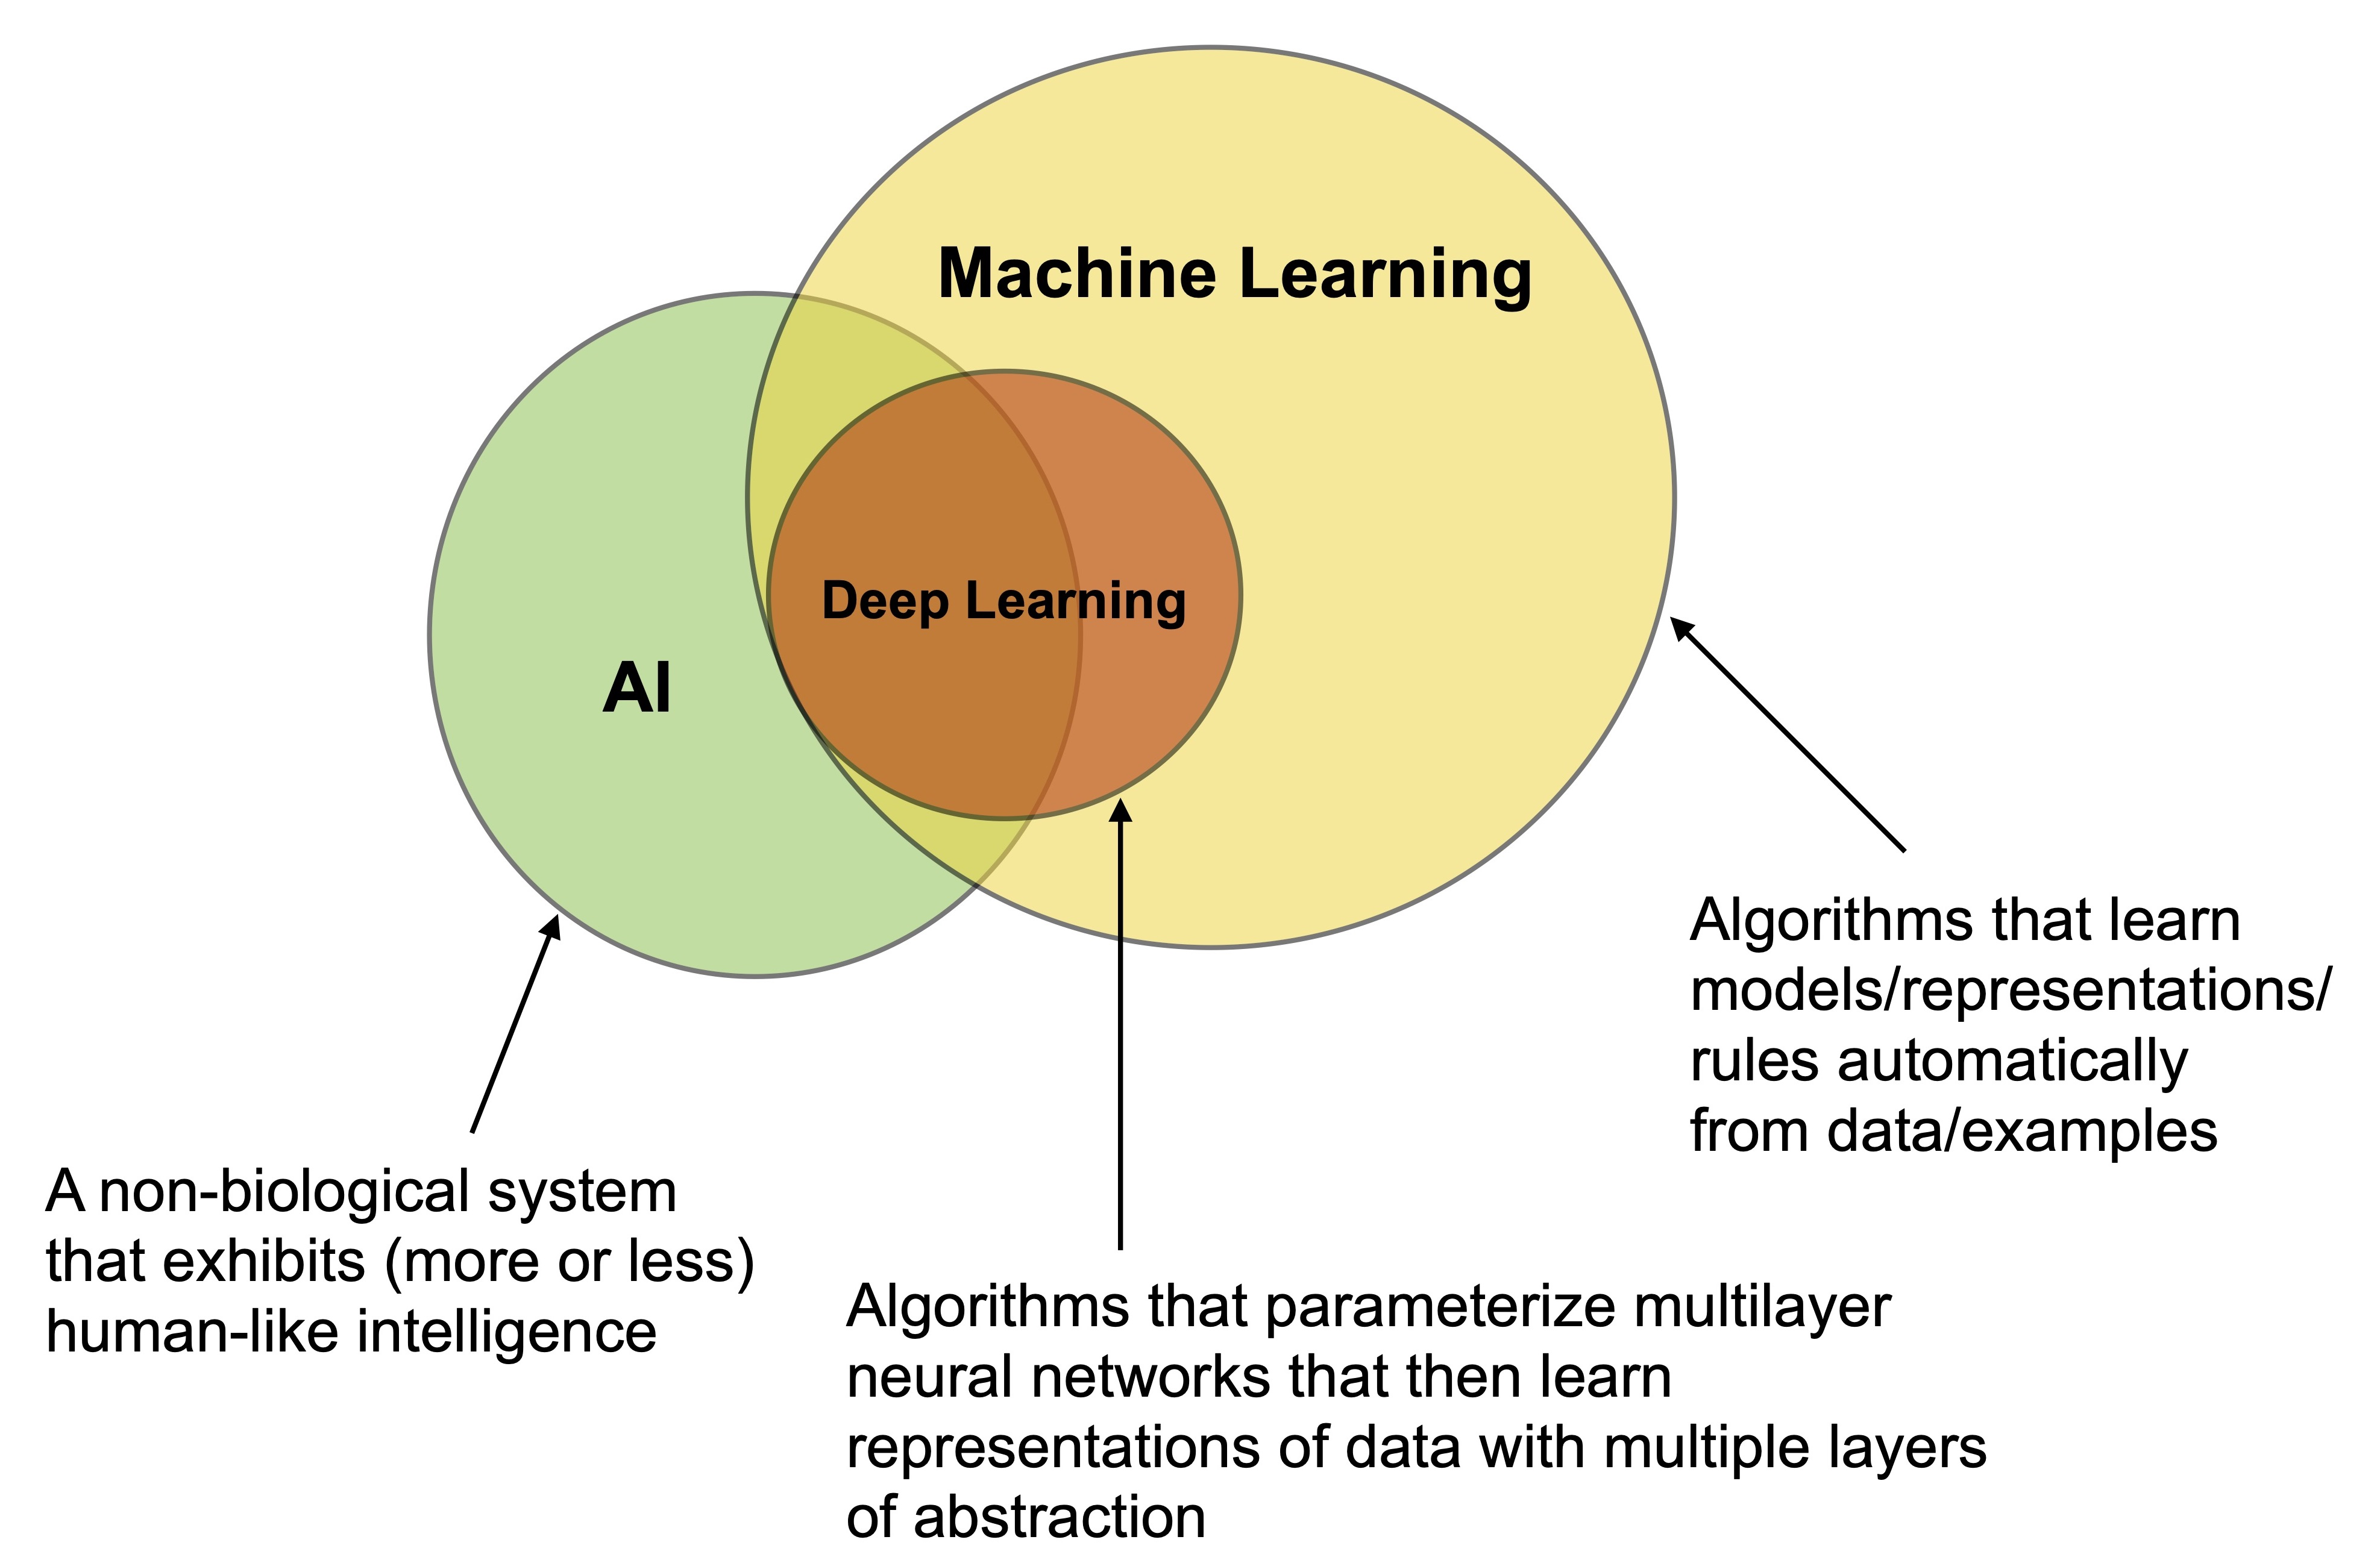
\includegraphics[width=\linewidth]{images/ai_ml_dnn_argue.jpeg}
        \caption[Overview of an alternative structure to the one used in this work for AI, machine learning, and deep learning.]{Overview of an alternative structure for \gls{ai}, machine learning, and deep learning. This structure argues that AI is the pursuit of developing non-biological systems with human-like intelligence and can be achieved with methods that do not use machine learning or deep learning, such as symbolic representations in a shallow architecture. This representation is not de facto and is not used in this work.\\Figure by Sebastian Raschka \cite{raschkaChapterIntroductionMachine2020}}
        \label{fig:ai_ml_dnn_argue}
    \end{figure} 

    \begin{figure}[htb]
        \centering
        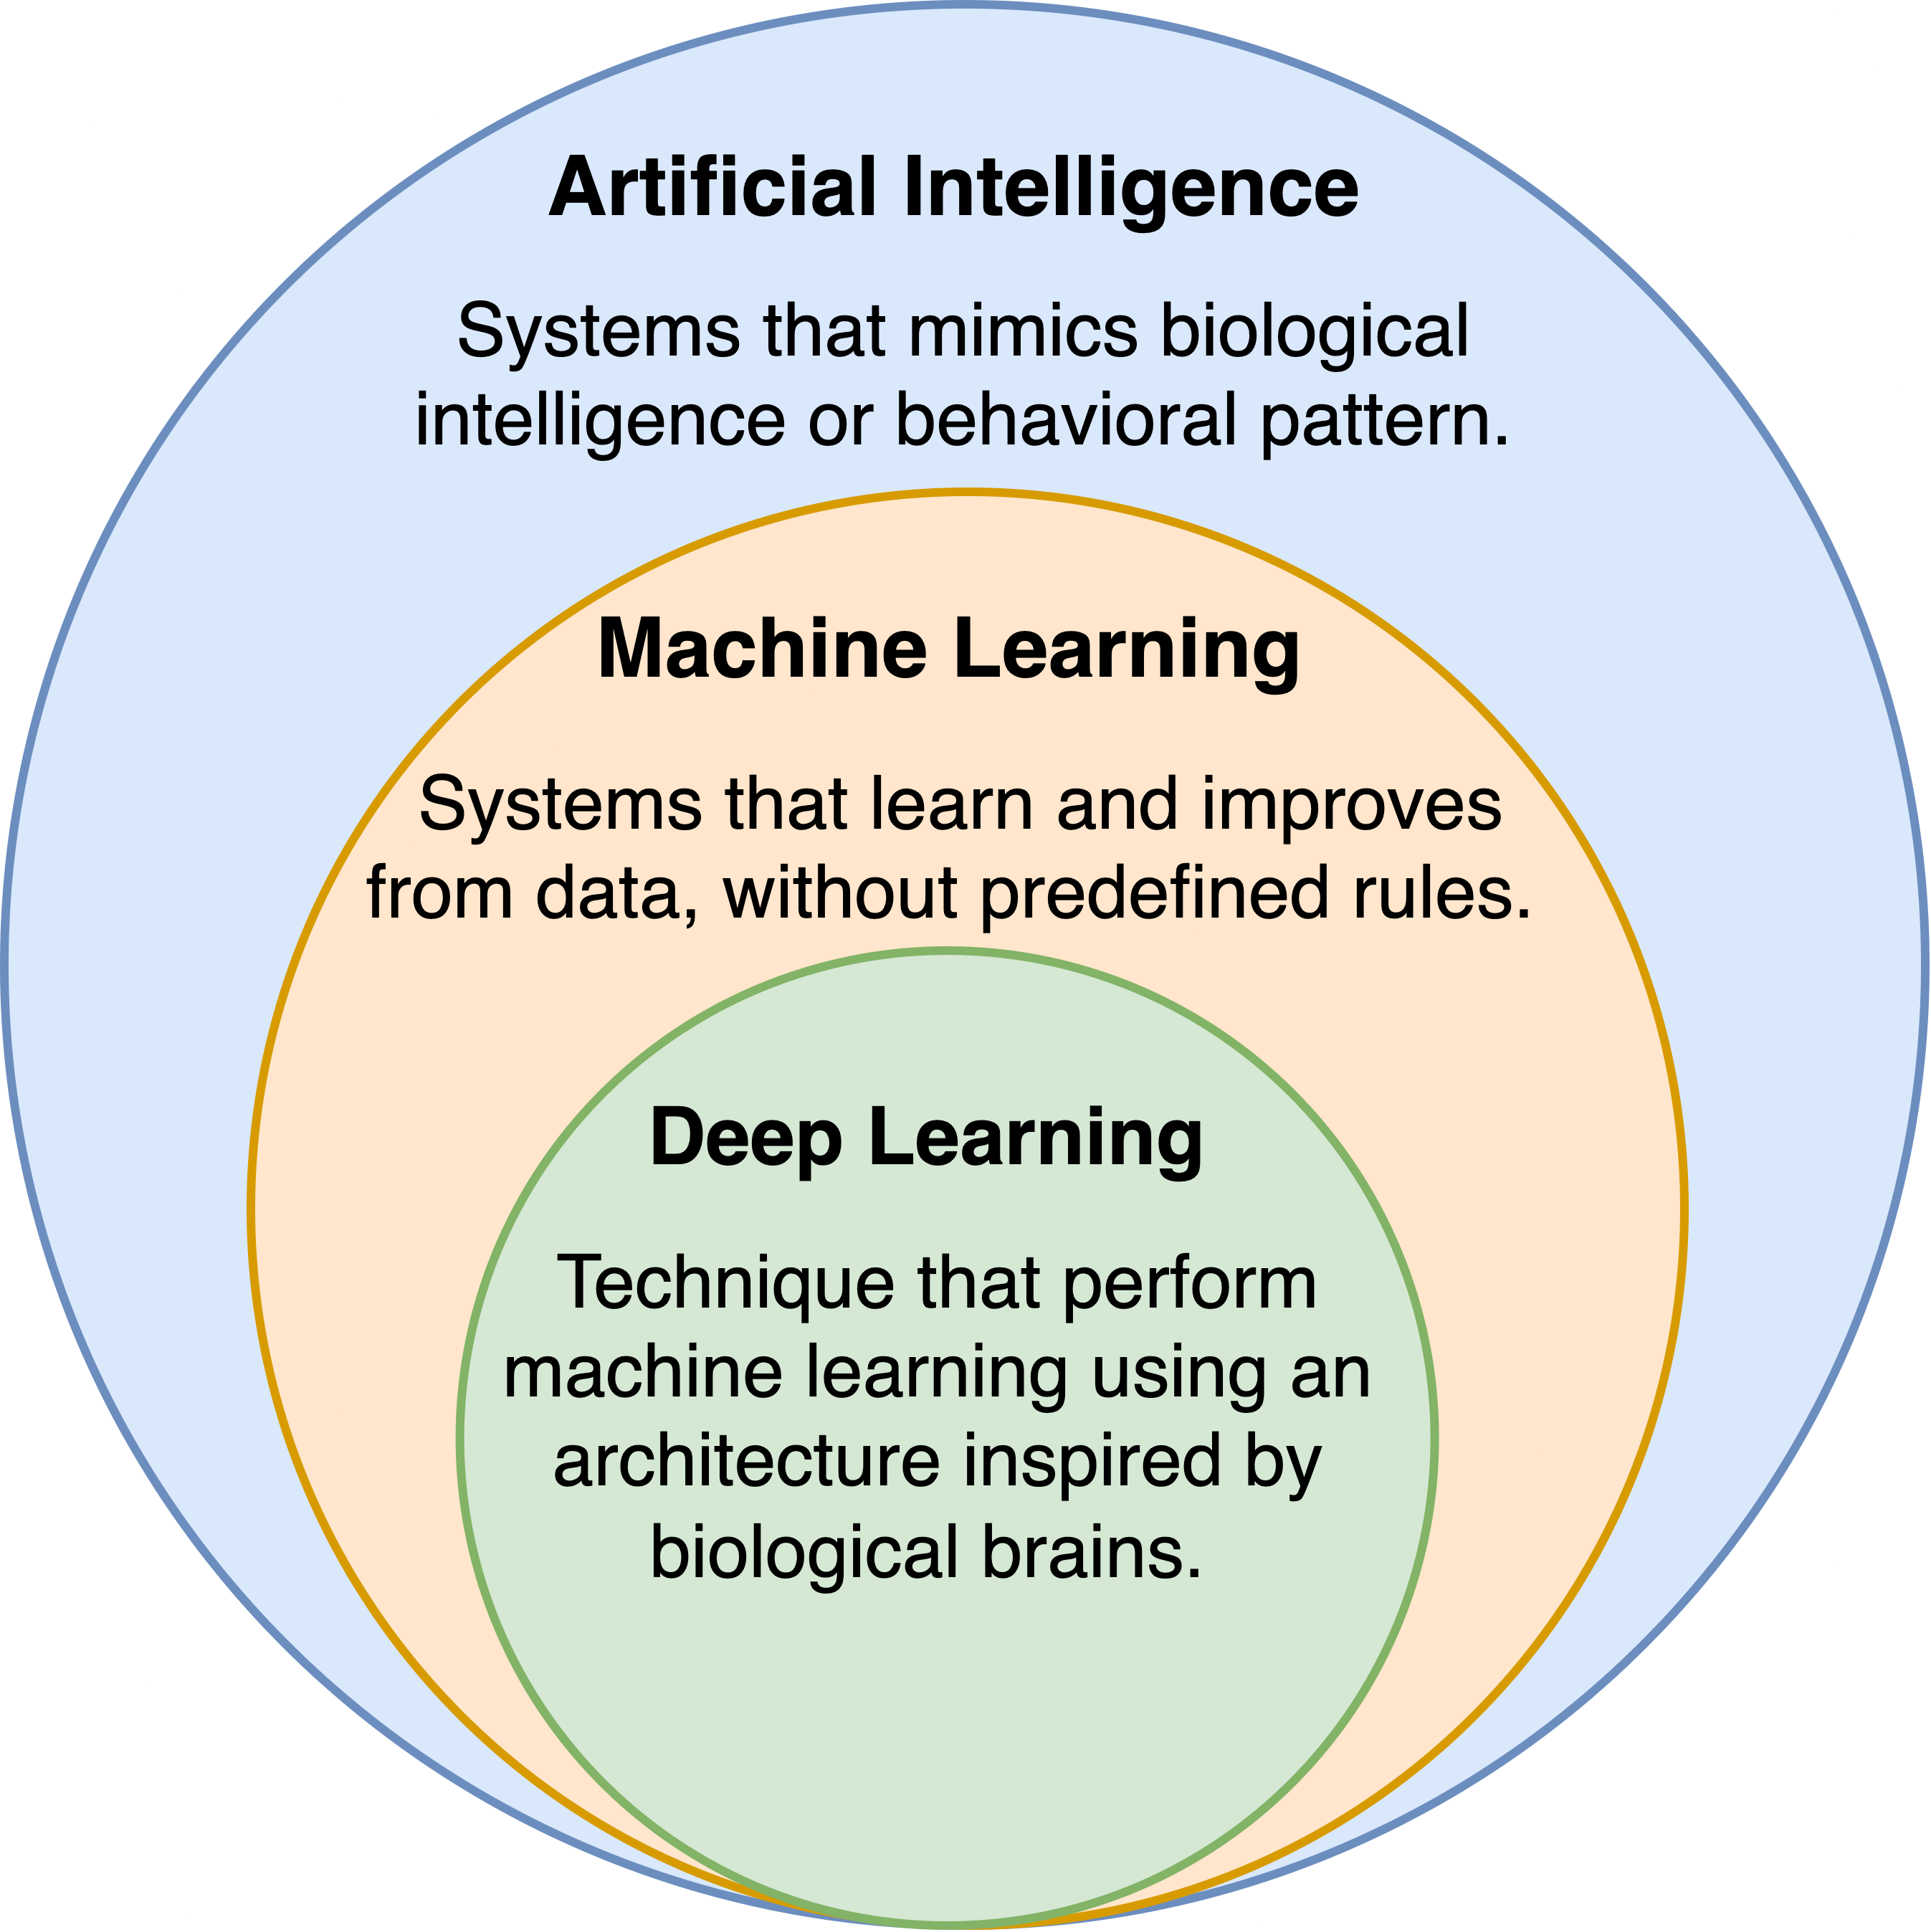
\includegraphics[width=9cm]{images/ai_ml_dnn}
        \caption[Overview of the structure between artificial intelligence, machine learning, and deep learning. This is the structure used in this thesis.]{Overview of the structure between artificial intelligence, machine learning, and deep learning. This is the structure used in this thesis.% Figure by the author.
        }
        \label{fig:ai_ml_dnn}
    \end{figure} 

    Machine learning is often broken down into three sub-areas, which are discussed and explained in this sub-section, explaining how they work, under what circumstances each sub-area can be used to advantage, and the challenges each branch faces are highlighted.

        \subsubsection{Supervised Learning}

        The first category within machine learning is known as supervised learning. This method is conceptually similar to using flashcards for memorization.
        The participant draws a card and reads the question while keeping the answer hidden. Only after the participant answers the question, the correct answer can be revealed. This is, in essence, the same approach used in supervised learning.
        
        
        In supervised learning, a dataset with pre-labeled examples, also known as a fully labeled dataset, is used to train algorithms to predict labeling for unlabeled input data. This is typically accomplished by training on a larger dataset with labels for each input, passing the input through a network, and using the label to inform the algorithm what the input data should be labeled as. In this way, the method learns the relationship between the input and the correct label. The method learns these correlations by adjusting the weights within the network to produce a result that is as close as possible to the true label.
        
        Since the ground truth label is known for each entry in the dataset, the model's output is compared to this ground truth label. The accuracy of the similarity between these two is measured using a loss function. 
        A loss function is a calculation that computes the loss of a single model prediction. The loss is a measure of how far from the ground truth the prediction was and is used to adjust the model to predict better next time. 
        Weights are adjusted using a technique called backpropagation to minimize this loss, and training continues until the weights are appropriately adjusted to achieve a satisfactorily low loss. These weights are then used later when testing real-world inputs, for which ground truth is often unavailable and must be estimated.
        
        Within supervised learning, there are two main subcategories: classification and regression. 
        
        Classification is a method used when the output variable belongs to a category, such as a color or an object, or to indicate the probability that an input belongs to one or more categories. Classification either predicts categorical class labels or classifies data by building a model. A typical classification method can be used to sort emails into spam or not spam or to identify the bird species in an image. Classification models can include methods such as neural networks, \gls{svm}, \gls{knn} \cite{fixDiscriminatoryAnalysisNonparametric1989, coverNearestNeighborPattern1967}, random forest, decision trees, one-vs-rest, and naive Bayes. Section \ref{sec:2_background_theory_deep_learning_and_neural_networks} will go into more detail about neural networks, as this is a central method of machine learning and is relevant to this work, as it is used later in this thesis by the first proposed architecture in Section \ref{sec:3_proposed_architecture}.
        
        The second approach within supervised learning is called regression. This method is used when the output should be a real or continuous value. Regression is used to find the correlation between dependent and independent variables. There are many different models within regression, such as linear regression, logistic regression, and polynomial regression. It is common to use hyperplanes that fit the available data. Hyperplanes are defined as a subspace of a vector space and have one less dimension than the vector space they are inside. These planes, therefore, are used to make a cut in the feature space in order to separate data samples.
        Regression is often used to make forecasts based on past data, e.g., estimating real estate prices for an area or salary growth.


        \subsubsection{Unsupervised Learning}

        Unsupervised learning is a technique that uses raw data from a given dataset to identify patterns and relationships in unlabeled data, facilitating the grouping of each item into appropriate clusters. The essence of this approach is that it can autonomously analyze and group data without requiring human intervention to pre-label the data. Therefore, it is well suited for use in data analysis, image recognition, and image segmentation.

        
        
        The main grouping models used in unsupervised learning are clustering, association, and dimension reduction. Clustering aims to divide raw data into groups or clusters based on similar characteristics. An example of a cluster split is shown in Figure \ref{fig:knn}, demonstrated by the \gls{knn} method. Association rules, on the other hand, are a rule-based approach that attempts to uncover relationships between variables in a dataset. These associations can, for example, be used in recommendation models, where companies can identify correlations between customers who purchase different items and use this knowledge to suggest similar products to new customers.

        \begin{figure}[htb]
         \centerline{
             \begin{subfigure}[b]{0.37\textwidth}
                 \centering
                 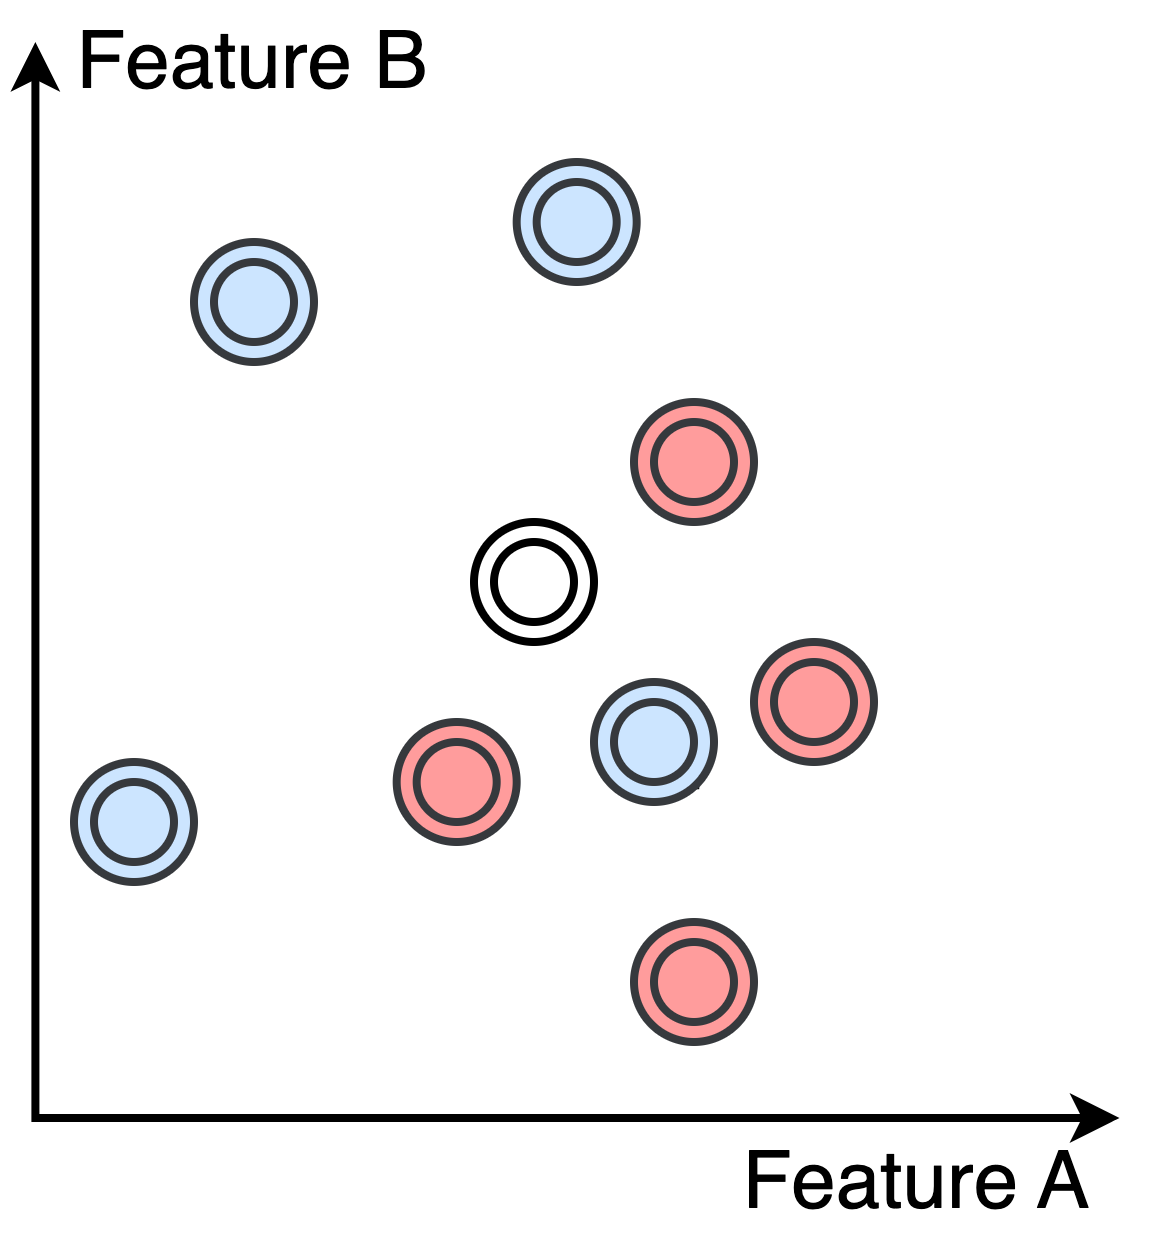
\includegraphics[width=\textwidth]{images/knn_1}
                 \caption{Samples are distributed in a feature space. The colors represent class, and the white is a new sample. A new sample will be classified based on neighboring samples.}
                 
             \end{subfigure}
             \hspace{0.015\textwidth}
             \begin{subfigure}[b]{0.37\textwidth}
                 \centering
                 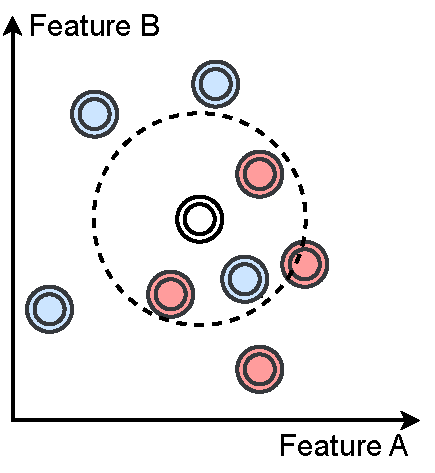
\includegraphics[width=\textwidth]{images/knn_2}
                 \caption{The new sample checks the nearest neighboring samples. In a circumference, noted with a dotted circle, the 4 closest neighboring samples are found.}
                
             \end{subfigure}
             \hspace{0.015\textwidth}
             \begin{subfigure}[b]{0.37\textwidth}
                 \centering
                 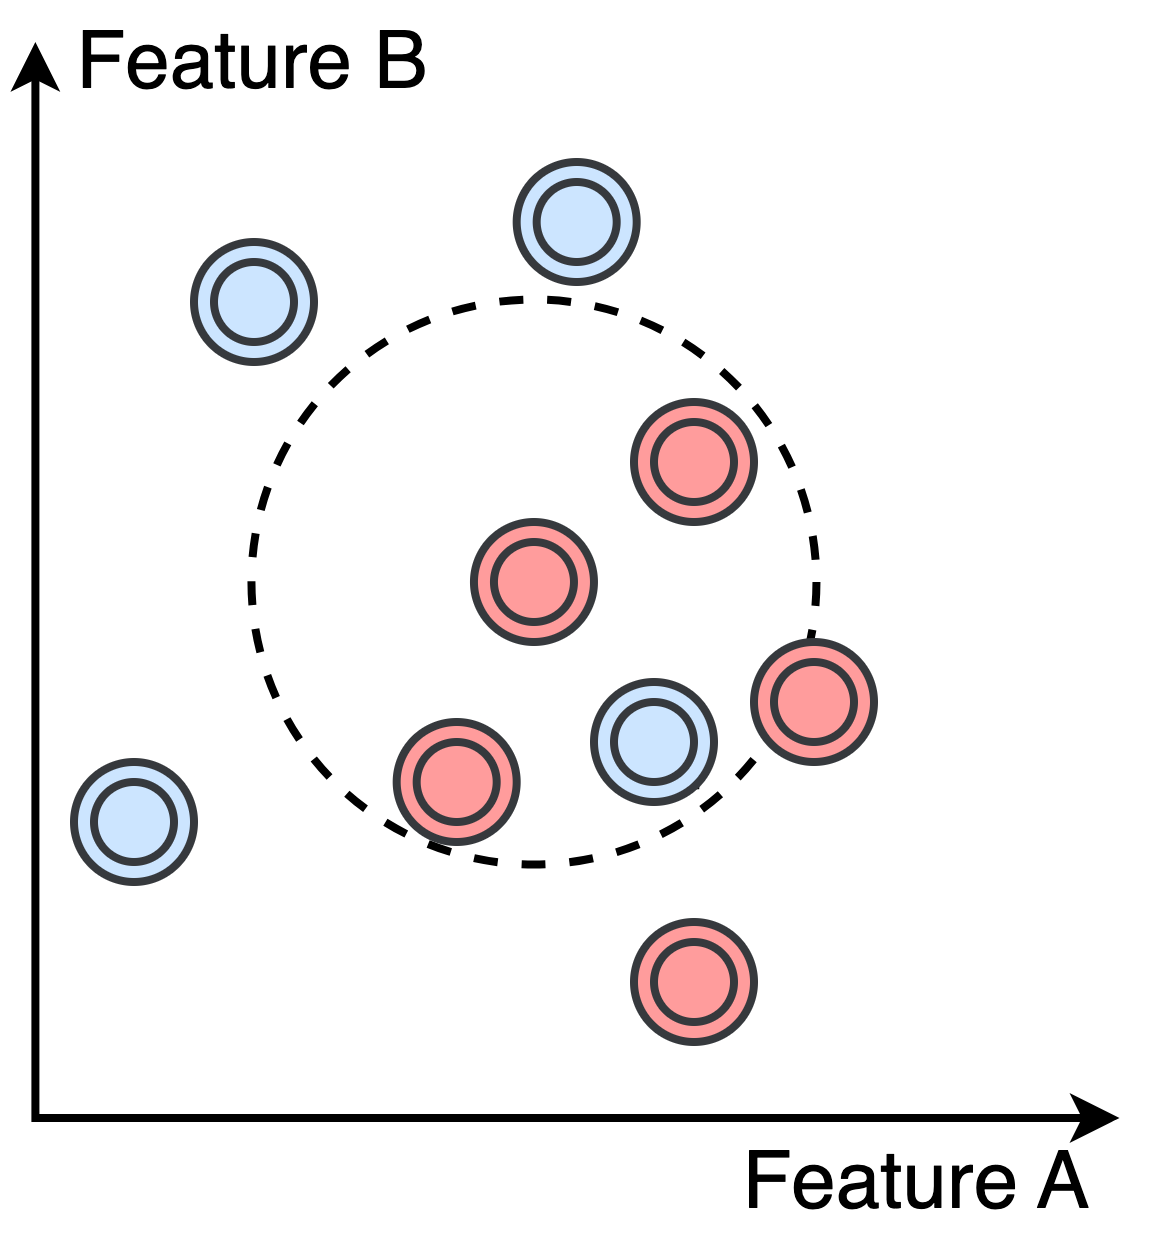
\includegraphics[width=\textwidth]{images/knn_3}
                 \caption{The classes of the 4 closest samples are counted, and the majority class is chosen. Of the 4 samples, one is blue, and three are red. The new sample is therefore classified as red.} 
             \end{subfigure}
             }
            \caption[Figure showing k-Nearest Neighbors clustering.]{Example of how the clustering algorithm k-Nearest Neighbors computes the class of a new sample. 
            %Figure by the author.
            }
            \label{fig:knn}
        \end{figure}
        
        Dimensionality reduction is a technique for reducing the number of dimensions in a dataset. 
        Although many machine learning methods benefit from additional data, this is not always the case \cite{belkinReconcilingModernMachinelearning2019, nakkiranDeepDoubleDescent2021}. Data samples can often contain insignificant variables or noise, making model training ineffective and making the dataset in practice smaller regarding useful information. This technique can be used to create a dataset containing more distinct features and also visualize and analyze data. When reducing the dimensions of a dataset, the goal is to reduce the number of learnable parameters while maintaining the integrity of the data being processed. Well-known methods for dimension reduction are \gls{pca} and \gls{svd}. More recently, good results have been obtained with deep neural network-derived autoencoders \cite{sakuradaAnomalyDetectionUsing2014}. Autoencoders can compress data fed to them and produce a representation or encoding that retains much of the underlying data, but the dimensions are significantly reduced.
        To retrieve this data after encoding, a decoder is required to reconstruct the data. Figure \ref{fig:auto_encoder} depicts an autoencoder with an encoder and decoder.

        \begin{figure}[htb]
            \centering
            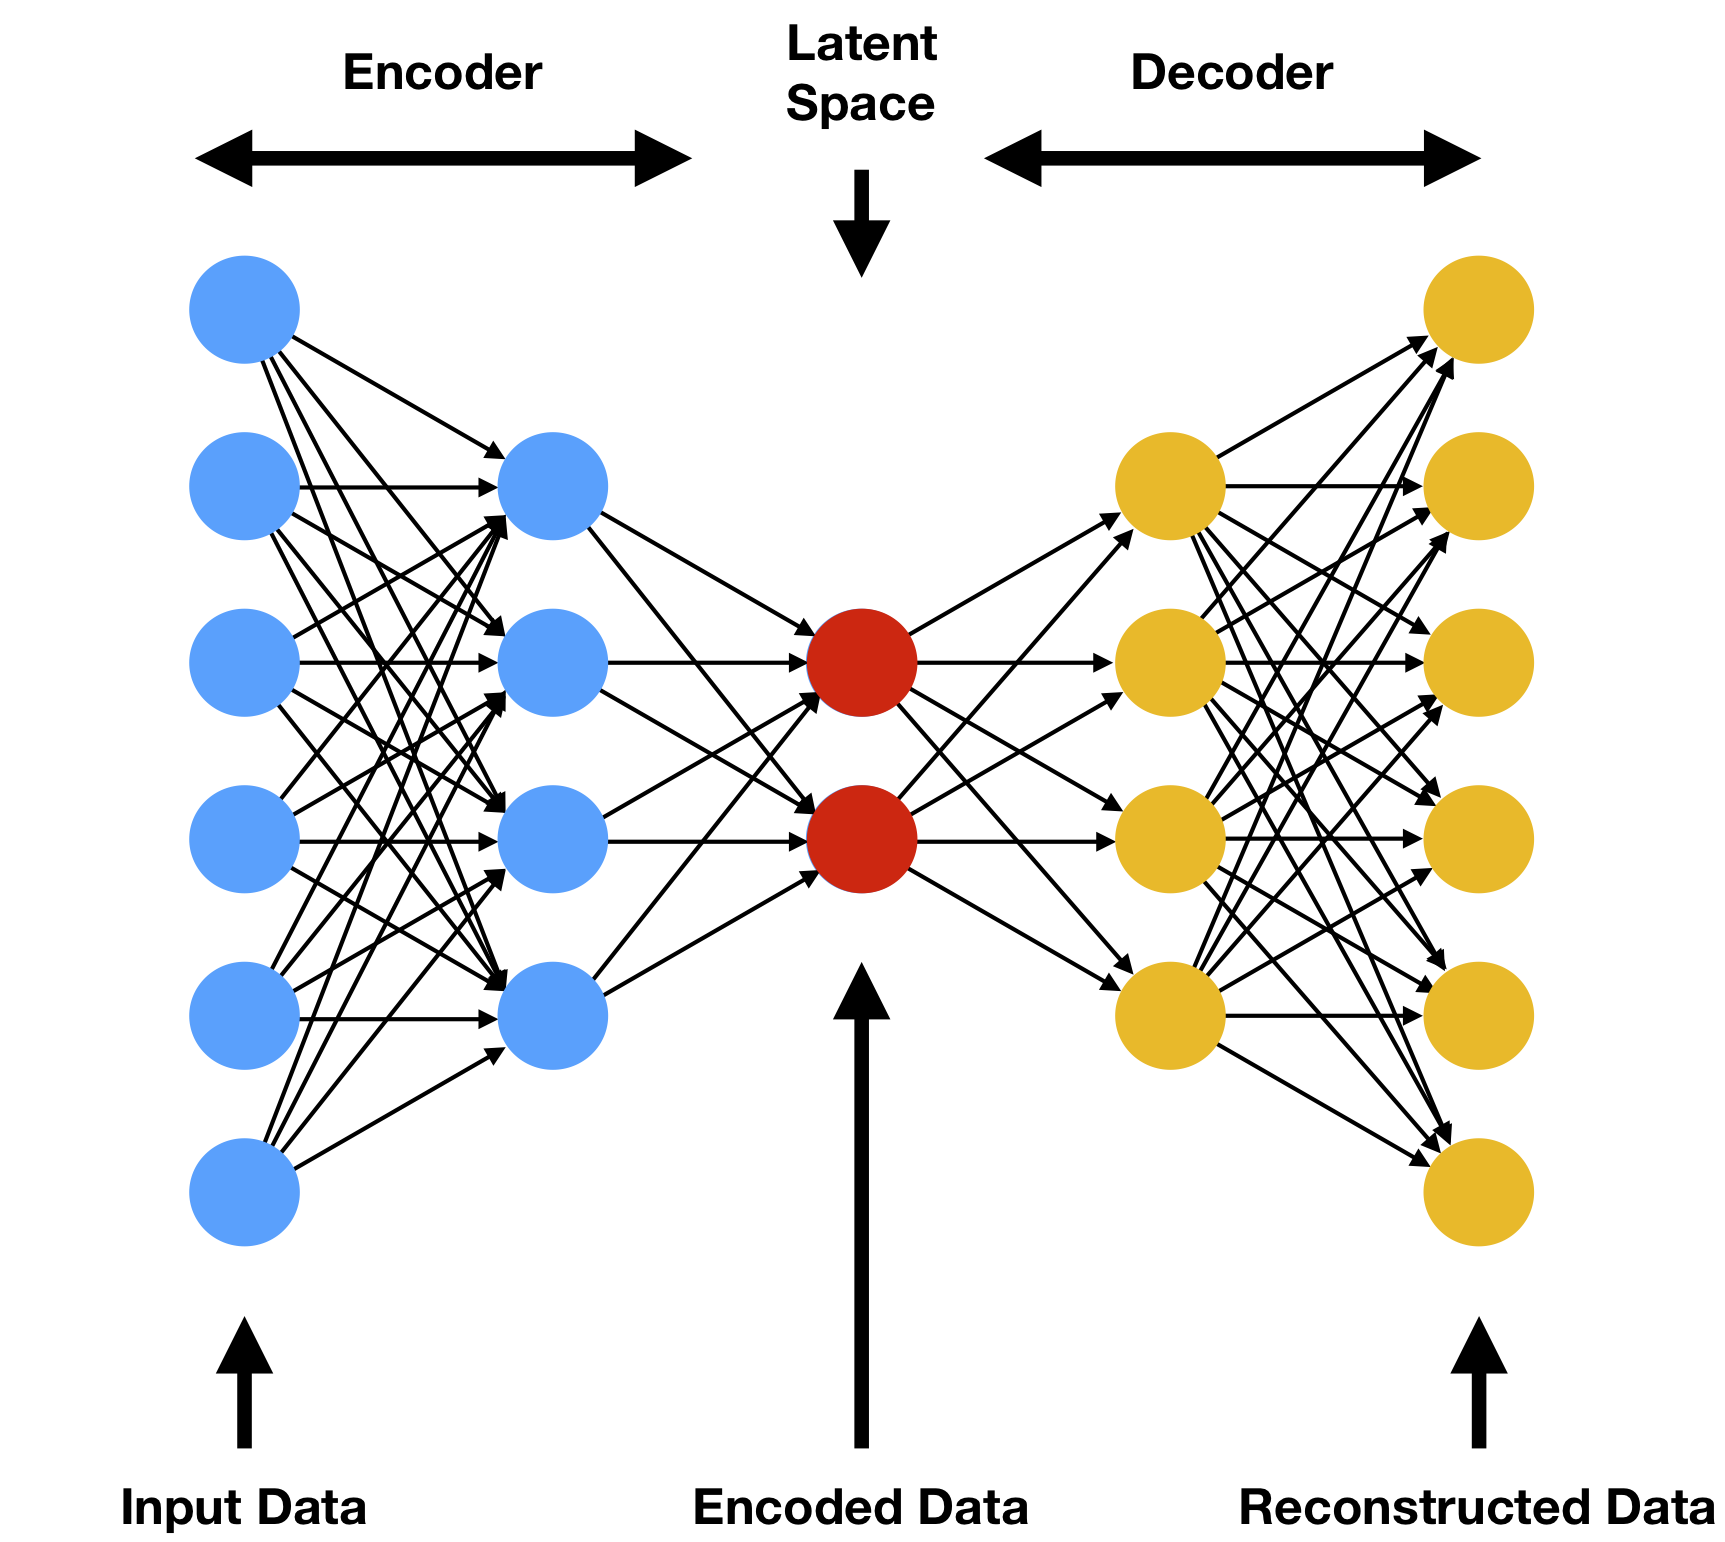
\includegraphics[width=\textwidth]{images/auto_encoder}
            \caption[Figure of an autoencoder.]{A diagram of an autoencoder consisting of an encoder and a decoder network. The encoder network maps the input image into a low-dimensional representation, while the decoder network reconstructs the original image from the low-dimensional representation. By minimizing the reconstruction error between input and output, the autoencoder can learn a compressed representation of the input data.\\Figure inspired by Steven Flores \cite{floresVariationalAutoencodersAre2019}.}
            \label{fig:auto_encoder}
        \end{figure} 
        
        Unsupervised learning has proven useful in computer vision, where it can aid in object recognition, detection, and segmentation, such as in medical datasets. By allowing correlations to be identified and grouped into clusters based on features or traits, unsupervised machine learning can also be used for anomaly detection, where it can flag atypical data. This method is also often used in recommendation engines, such as those found in online stores, streaming services, or social media.


        \subsubsection{Semi-Supervised Learning and Hybrids}

        % https://en.wikipedia.org/wiki/Semi-Supervised_Learning#Semi-supervised_learning
        % https://en.wikipedia.org/wiki/Active_learning_(machine_learning)
        % https://ai.stanford.edu/blog/weak-supervision/
        % https://medium.com/geekculture/weak-supervision-and-active-learning-352fe8dc7df8
        % https://snorkel.ai/weak-supervision/
        % https://www.youtube.com/watch?v=SS9fvo8mR9Y
        % https://www.youtube.com/watch?v=-cc2RYF37zE

        Supervised learning is often more accurate than unsupervised learning as it can learn from the knowledge provided by humans in the form of labeled data. This approach can also avoid computational complexity since the model does not need to train on irrelevant features for the specific task. However, the downside of supervised learning is that it requires significant human effort beforehand labeling the dataset, which can be time-consuming and costly, particularly when domain experts are required.

        A hybrid solution that aims to leverage the best of both supervised and unsupervised learning is known as semi-supervised learning. This approach can be beneficial when there is too much data to label, either because the dataset is large or the cost of labeling is high. Semi-supervised learning typically assumes that data points close together in feature space share labels or have an underlying correlation factor in a lower dimension (manifold hypothesis/assumption). Methods using semi-supervised learning often achieve higher accuracy than those using only supervised or unsupervised approaches separately. This is because they do not need to discard data that is not labeled and can be trained using a researcher's \textit{a priori} knowledge of the dataset or possible solution \cite{reddySemisupervisedLearningBrief2018, berthelotMixMatchHolisticApproach2019}.
        
        Other approaches, such as active learning and weak supervision, can also often be used when a fully labeled dataset is unavailable for training. Active learning is a process in which a model can select input data about which it is unsure and ask a human or other expert for the correct answer. For example, such methods can label large data sets with services such as Amazon Mechanical Turk \cite{AmazonMechanicalTurk}. Samples are selected using a model that attempts to ask for samples believed to have the highest value for further classification. This can be achieved by first asking an expert for a sample from random samples and fitting the model to obtain a decision boundary that separates the classes. After that, the model can iteratively identify examples of high importance since they are near or at this decision boundary. These are the most uncertain examples, making them valuable for the model to identify. Then the model asks the expert for samples near the boundary. The boundary is adjusted again, and the process is repeated until the model fits the data and satisfactorily separates the samples.
        
        Weak supervision is a method that can be applied in situations where it is preferable to have a large number of sufficiently accurate examples rather than a smaller number that are completely correct \cite{hoffmannKnowledgeBasedWeakSupervision2011}. This approach is often implemented by defining some rules or using a knowledge base in advance, which helps the model estimate the probability that an example belongs to a certain category. Weak supervision is often used in conjunction with transfer learning, which involves transferring knowledge from one area to another \cite{wangSimVLMSimpleVisual2022}. Transfer learning has shown promising results because generalizable knowledge of data can often be transferred, eliminating the need to learn from scratch on a new dataset. Transfer learning can be combined with other methods, e.g., supervised learning \cite{zhuangComprehensiveSurveyTransfer2021}.
    
    \subsection{Deep Learning and Neural Networks} \label{sec:2_background_theory_deep_learning_and_neural_networks}
    Neural networks, also known as \glspl{ann}, are a machine learning method inspired by how the biological brain processes information and learns. Essentially, \glspl{ann} approach the goal of extracting information and constructing knowledge by forming a network of artificial neurons that can process input data. These artificial neurons, called perceptrons, are the building blocks of neural networks and are likewise inspired by biological neurons. In this representation, the inputs to the artificial neuron are synapses on the dendrites, the axon hillock inspires the activation function, and the output from the artificial neuron is the biological axon.
    
    The artificial neurons process data by weighting the input data and a predetermined bias before passing it through an activation function, such as a sigmoid or \gls{relu} \cite{dubeyActivationFunctionsDeep2022} that produces the neuron's output. When the output of the activation function exceeds a certain threshold, the neuron is activated and sends data to the next layer. No further data is sent if the output does not exceed the threshold.

    \begin{comment}
    % Remove this
    This processing step of a perceptron can be viewed as a linear regression, as in shown formula ?. However, unlike linear regression, perceptrons in \glspl{ann} are connected in a network, so changes in weights cascade to the next level of perceptrons. A single-layered neural network can therefore be seen as a logistic regression function.
    \end{comment}
    
   \glspl{ann}, often called multi-layer perceptron (MLP), are the cornerstone of deep learning, which refers to \glspl{ann} with more than three layers. The smallest deep network, therefore, has an input layer, two hidden layers in the middle, and an output layer. These middle processing layers are called the hidden layer because it is hidden from the outside, which the input and output layers are not. An example of such a network with two hidden layers is shown in Figure \ref{fig:deep_network} to see. 


    \begin{figure}[htb]
        \centering
        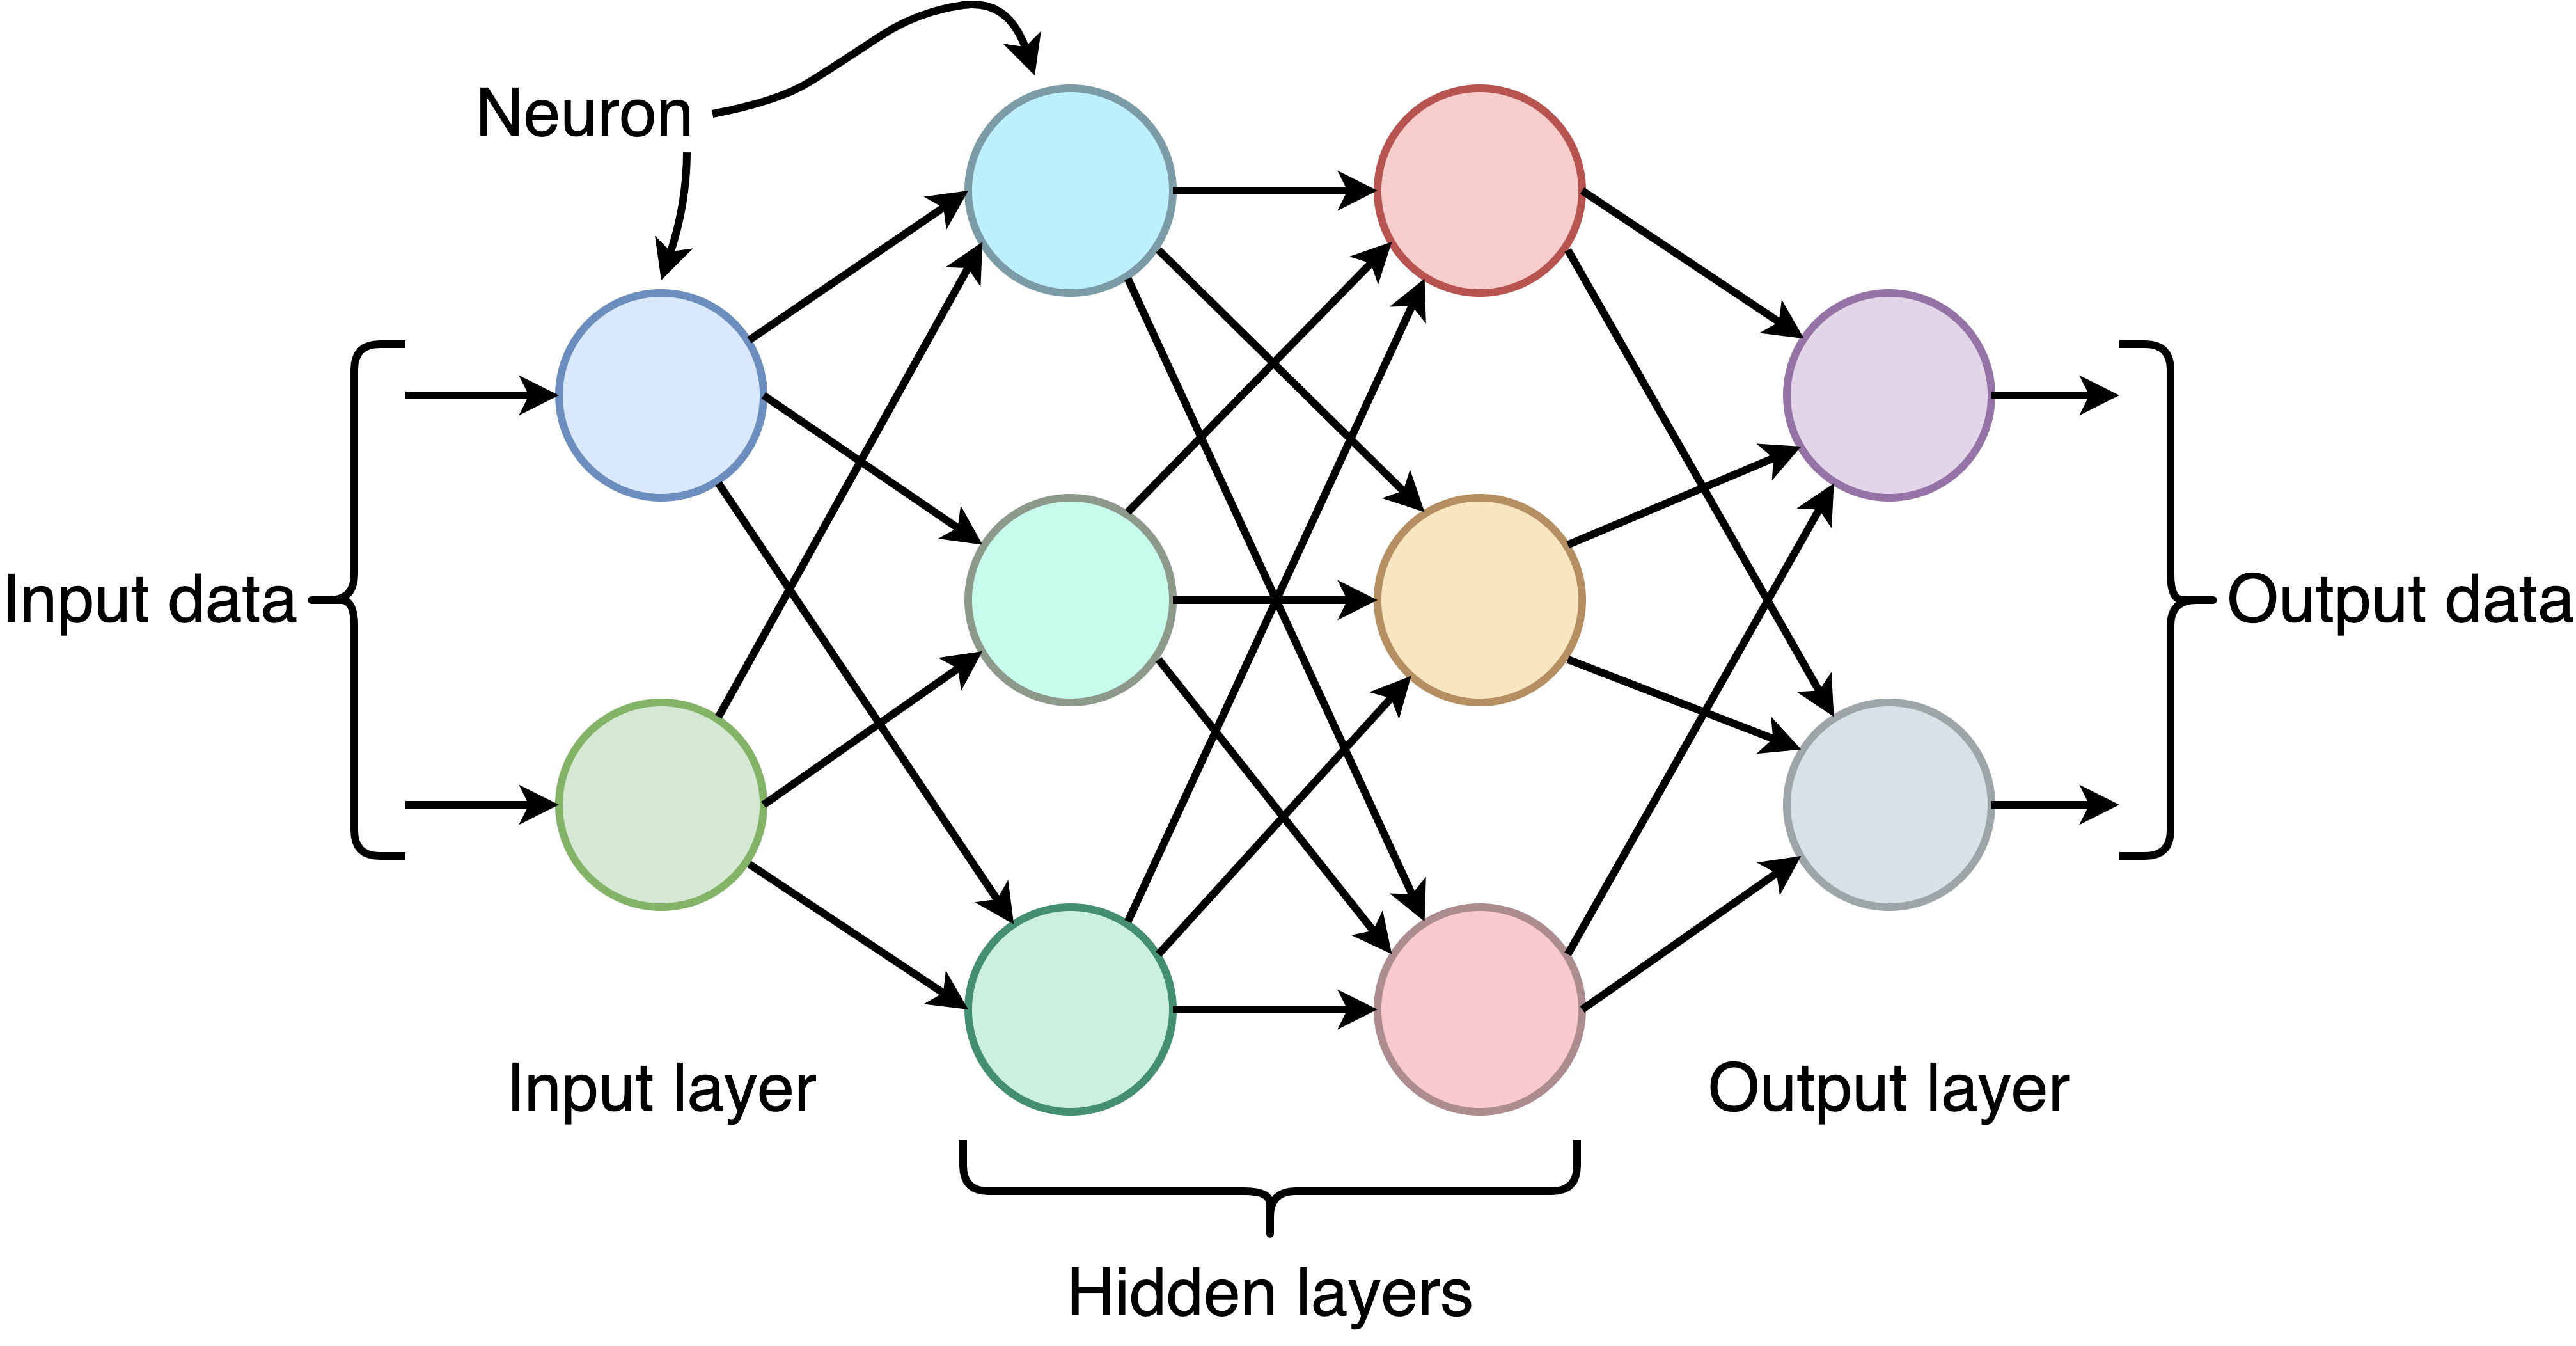
\includegraphics[width=\linewidth]{images/deep_neural_network}
        \caption[Figure of a fully connected deep artificial.]{A fully connected deep artificial neural network with two hidden layers and two input and output neurons.} %Figure by the author.}
        \label{fig:deep_network}
    \end{figure}

   
    
    Most \glspl{ann} are feedforward, meaning that data is entered on one side, passed through the network, and produces a result on the other end. These networks are often trained using backpropagation, where the network output is compared to the ground truth, and the difference between the estimated result and the ground truth is used to adjust the network weights to minimize this difference. The backpropagation technique is also inspired by biological backpropagation, which occurs when a neuron generates an action potential that sends a voltage spike back to the dendrites. Other methods are proposed instead of feedforward combined with backpropagation, such as the proposed forward-forward algorithm by Geoffrey Hinton \cite{hintonForwardForwardAlgorithmPreliminary2022}.


    Deep neural networks have achieved remarkable achievements, mainly due to their ability to learn from structured and unstructured data. This allows them to learn and generalize knowledge given sufficient amounts and high-quality data \cite{willeminkPreparingMedicalImaging2020}. Before computing power allowed deep networks, hand-made feature extractors were commonly used, using human-predefined features such as texture, shape, and color for object recognition tasks. However, when deep learning was first used in the \gls{imagenet} competition \cite{russakovskyImageNetLargeScale2015}, which is a competition identifying objects from the ImageNet dataset \cite{dengImageNetLargeScaleHierarchical2009}, it achieved great results as shown in Figure \ref{fig:imagenet_results_graph}. This figure shows the methods and their classification error for each year the competition was arranged. It is clear that deep learning made significant strides in 2012 with AlexNet, which was proposed by Krizhevsky et al. \cite{krizhevskyImageNetClassificationDeep2017}. These methods have improved significantly since then, largely thanks to improved methods and hardware. In 2015, deep learning even surpassed the human ability to classify images in ImageNet with the ResNet model proposed by He et al. \cite{heDeepResidualLearning2015, heDelvingDeepRectifiers2015}.
    
    \begin{figure}[htb]
        \centering
        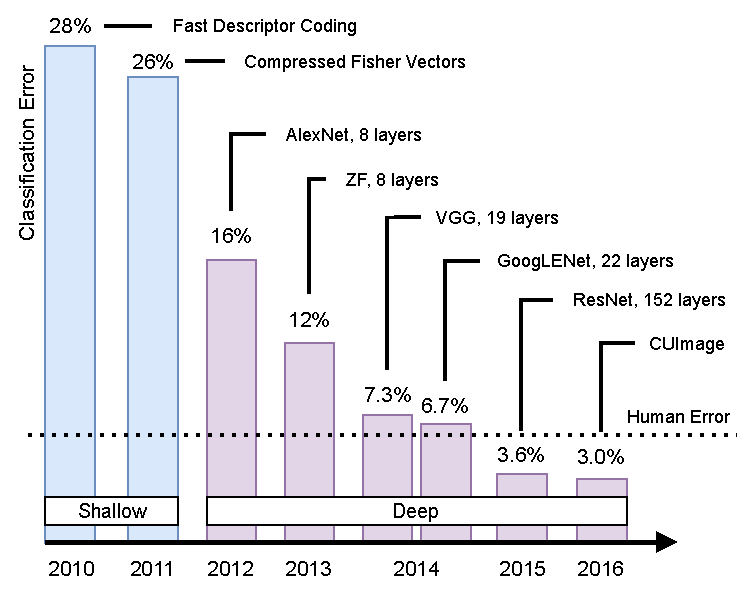
\includegraphics[width=\linewidth]{images/imagenet_results_graph}
        \caption[ImageNet competition winners from 2010 to 2016.]{Overview of the ImageNet competition winners from 2010 to 2016. The figure shows how deep networks have significantly improved the networks' ability to guess the right label for the images in the ImageNet dataset. In 2015, the deep network ResNet \cite{heDeepResidualLearning2015} surpassed the average human ability to label these images correctly. \\
        Figure inspired by Gordon Cooper \cite{cooperSoftwareFrameworkRequirements2017}.}
        \label{fig:imagenet_results_graph}
    \end{figure}


    
    \subsection{Convolutional Neural Networks}

    % Intro to CNNs
    Inspired by biology alongside regular neural networks, the computer vision method called \glspl{cnn} is designed to mimic how the brain's visual cortex processes visual information. \gls{cnn} builds on the idea and technique of neural networks and adds at least one convolutional layer. A convolutional layer allows information about neighboring entities to be obtained from the previous layer. The method has proven particularly effective in computer vision to process and analyze images and video because it can gather context from nearby areas where the convolution is centered. This can help the method extract contextual and semantic relationships that would otherwise have been lost. Both of the proposed methods presented in this thesis use a \gls{cnn}, namely a VGG-16 model \cite{simonyanVeryDeepConvolutional2015}, to classify images and extract image features. Therefore, understanding how \glspl{cnn} are constructed and their advantages and uses are relevant.

    % Intro to convolution layers
    The convolution layer works by scanning small filters across the input image, computing dot products between the filter and the image pixels at each location, and creating a feature map. A convolution layer can be considered a flashlight beam aimed at an image. The beam of light allows the viewer can see areas of the image that are in the perimeter of the area where the center of the beam is directed. As the beam of light moves across the image, the viewer can comprehend more of what is in the image. An illustration of a convolution is shown in Figure \ref{fig:convolutuon}.

    \begin{figure}[htb]
        \centering
        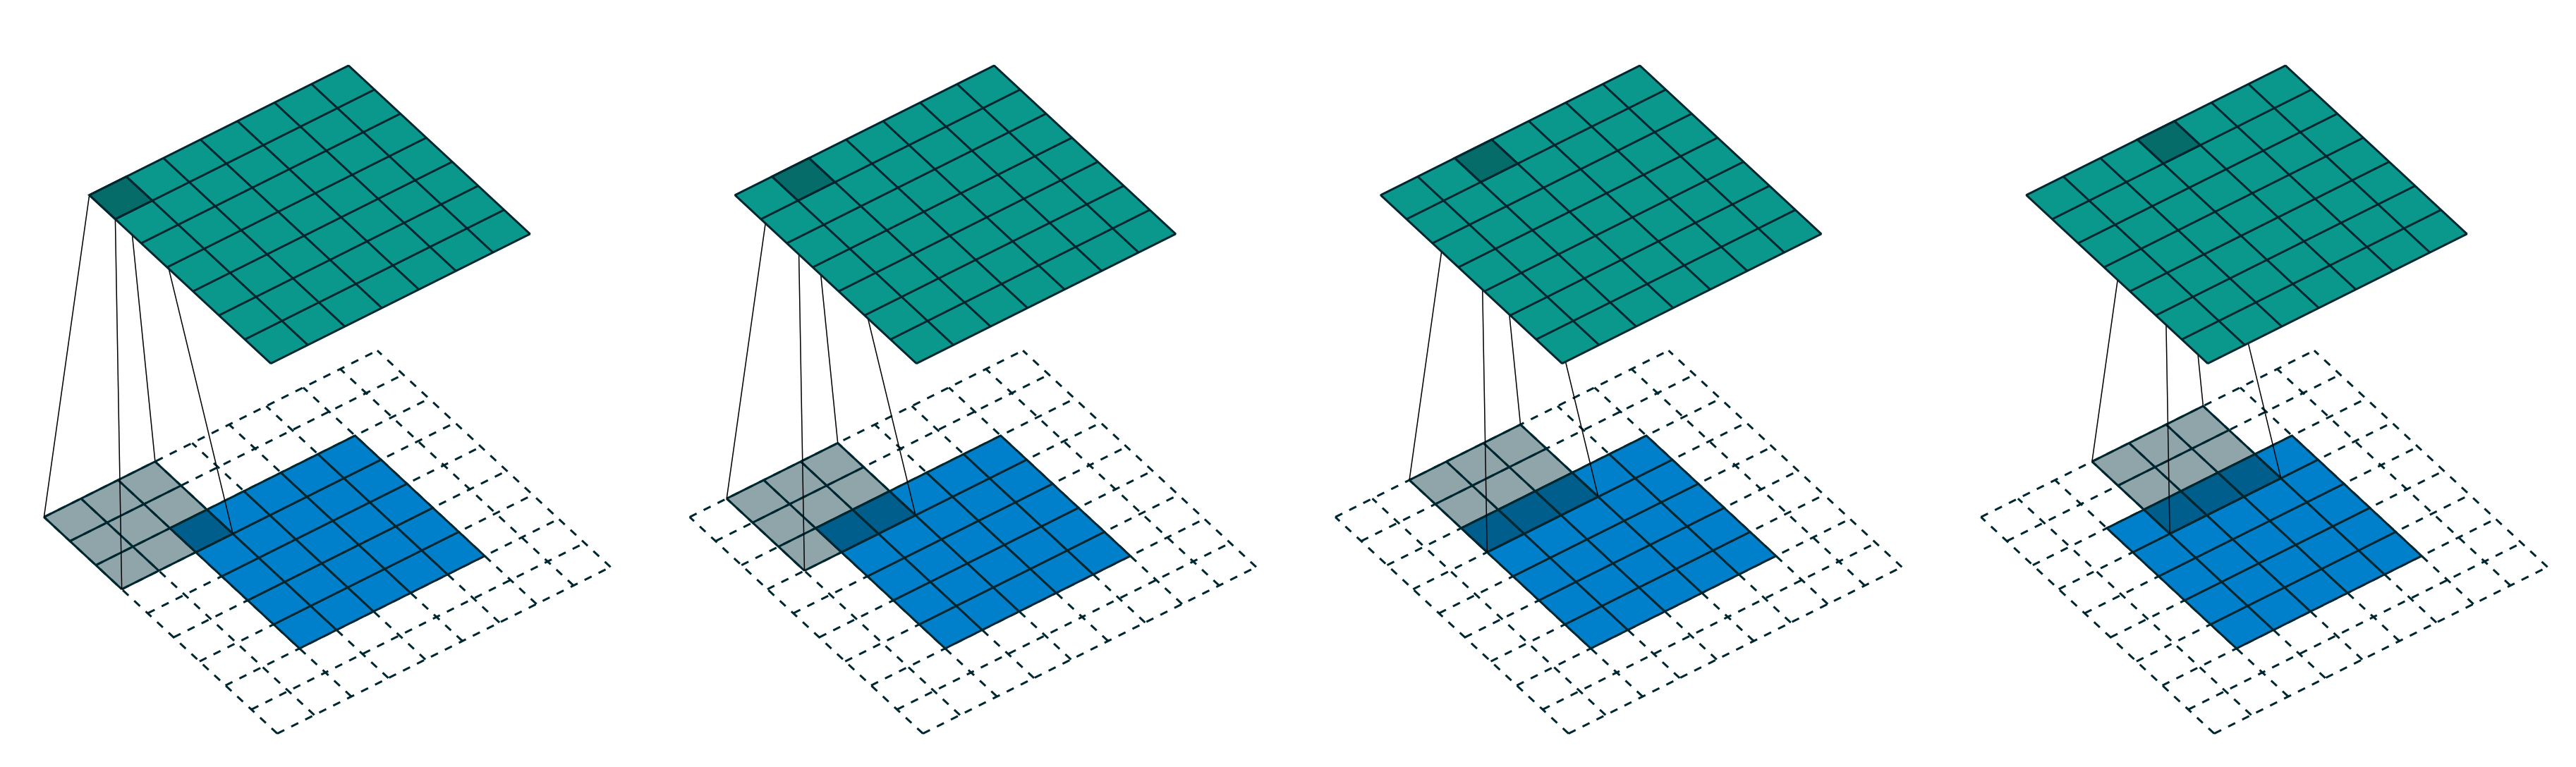
\includegraphics[width=\linewidth]{images/convolution.png}
        \caption[Illustration of a convolution.]{An illustration of a convolution where a $3 \times 3$ kernel is convolved with a $5 \times 5$ input matrix. The convolution illustrated has full padding and a one-step stride.\\
        Figure by Vincent Dumoulin and Francesco Visin \cite{dumoulinGuideConvolutionArithmetic2018}.}
        \label{fig:convolutuon}
    \end{figure}


    % Short history and advantage.
    The first \gls{cnn} that trained with backpropagation was first proposed by LeCun et al. in 1989 \cite{lecunHandwrittenDigitRecognition1989} and has since had a huge importance in making machines interpret images and videos. A major advantage of using a convolutional layer is that it can compress information while preserving information and the context around the retrieved information. A very common \gls{cnn} architecture is shown in Figure \ref{fig:vgg_cnn}. Also seen in the figure is that a typical \gls{cnn} has a fully connected neural network. A \gls{cnn} often uses fully connected layers, unlike a normal neural network, because of the condensation of information with surrounding information, allowing for a network that can take advantage of using many parameters without overfitting.  

    \begin{figure}[htb]
        \centerline{
        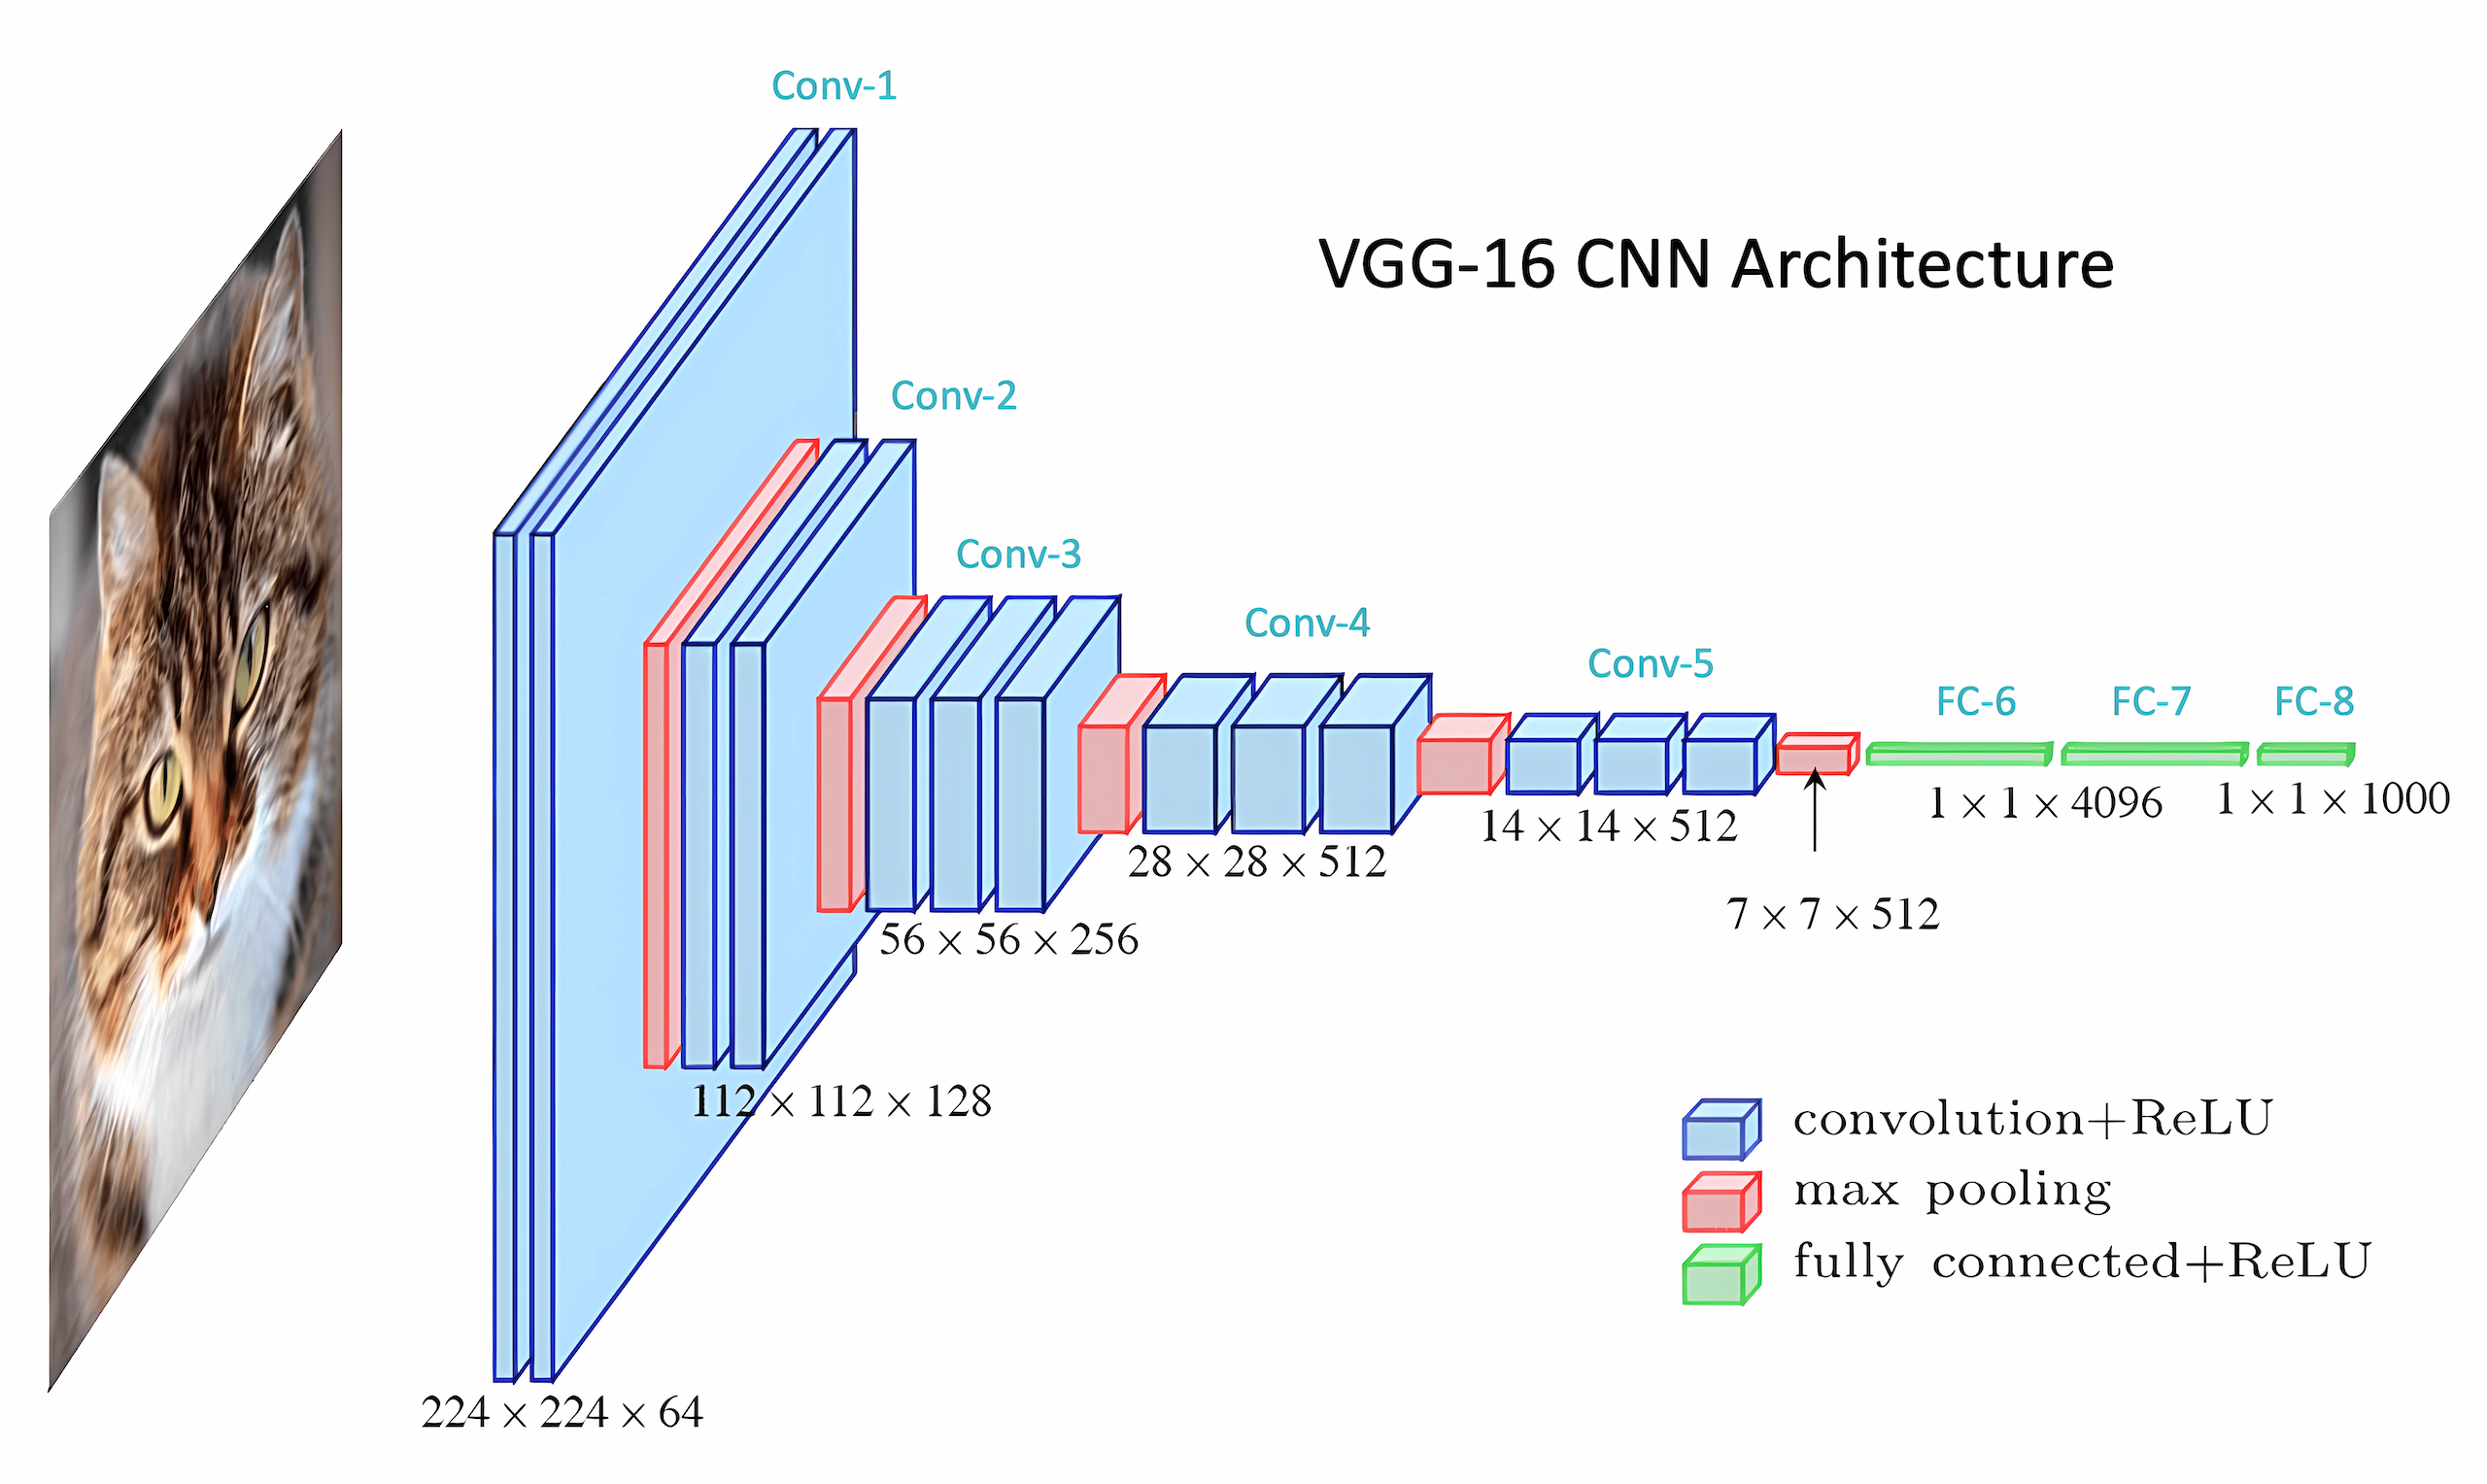
\includegraphics[width=1.1\linewidth]{images/vgg_cnn.png}}
        \caption[Example of a CNN architecture, illustrated by the VGG-16.]{Example of a typical CNN architecture, here illustrated by the VGG-16 model proposed by Simonyan and Zisserman \cite{simonyanVeryDeepConvolutional2015}. As seen in this figure, the first part of the network convolves the input image and extracts feature maps. These feature maps are then fed into a fully connected artificial network that classifies the image in a given class.\\
        Figure by Satya Mallick \cite{UnderstandingConvolutionalNeural2023}.}
        \label{fig:vgg_cnn}
    \end{figure}
    
    The convolution layers can be applied to an input image as a series of filters, producing a series of feature maps that emphasize different aspects of the image. These filters have weights that are learned and adjusted during training and are able to recognize different types of patterns of increasing complexity and abstraction from the input image. The training process is similar to regular neural networks. It typically updates weights using backpropagation to minimize the loss function and improve the accuracy of the network on the training set. The first layers, closest to the input image, generally recognize low-level features such as edges, lines, corners, texture, and color. As the convolutional layers process the input information, more complex features can be detected that build an abstraction on the information extracted from earlier layers. Convolution layers farther from the image can recognize more high-level features such as shapes, objects, and scenes. Overall, the convolutional layers allow the features of the input image to be analyzed hierarchically, with the early layers capturing low-level features and the later layers capturing high-level features.
    
    % More in-depth architecture with pooling layers.
    \glspl{cnn} are typically designed with multiple layers, similar to deep neural networks, and the last layers are typically fully connected. The fully connected layers take the output of the convolution layers, a set of feature maps, and convert them into a single vector of class scores that represent the probability that the input image belongs to each possible class. The main function of pooling layers in \glspl{cnn} is to reduce the spatial dimensions of the feature maps generated by convolutional layers while preserving the most salient features of the input image. Pooling layers operate on small regions (e.g., 2x2 or 3x3) of the feature maps generated by the previous convolution layers and reduce their size by applying a pooling function, such as max pooling or average pooling, on each region. Max pooling selects the maximum value within each region as the representative value, while average pooling calculates the mean of the region. These operations effectively downsample the feature maps and help reduce the network's sensitivity to small spatial translations and variations in the input. Pooling layers can be inserted after one or more convolutional layers in a \gls{cnn}. Their hyperparameters, like the size of the pooling area and the stride (i.e., the amount of movement of the pooling window), can be tuned to control the amount of downsampling and the size of the resulting feature maps.
    
    Additionally, pooling layers can prevent network overfitting by reducing the number of parameters and the computation time required for training. The role of pooling layers in \glspl{cnn} is not limited to downsampling. However, they can also help to capture translation invariance, i.e., the property that the learned features are invariant to small translations in the input. The translation invariance is achieved because the max or average operation selects the most prominent feature in a given region, regardless of its exact position. This property allows the network to collect more general relationships in the input data, providing a more general understanding of the network. The overall benefits of pooling layers lie in reducing the spatial dimensions of feature maps while preserving their salient features, resulting in more efficient and robust image analysis.
    
    % Summary
    In essence, the different layers of a \gls{cnn} work together to extract and classify features in images and videos. This makes \glspl{cnn} particularly effective for tasks such as image classification, object detection, and segmentation, where detecting and locating different features of an image is critical for accurate performance. \glspl{cnn} have proven highly effective in image classification tasks, outperforming other types of neural networks and traditional machine learning algorithms. They have been used in various applications, including object recognition, facial recognition, and medical image analysis. With the development of larger and more complex networks and the availability of powerful hardware and software, \glspl{cnn} remains an active area of research and development in machine learning.


\section{Image Captioning}

    The methods proposed in this thesis use techniques to extract information from input images and present a text output. The method to make a model give a textual description to an image is often called image captioning.
    Image captioning is a field of research where the objective is to generate textual descriptions using natural language from the content of an image. This process uses computer vision and \gls{nlp} to gather information from images and give a text that describes or analyzes the image's content. Image captioning is, therefore, a multimodal method that has excelled with the advancements in computer vision, helped considerably by \glspl{cnn} and language models. The motivation for developing this field of research is that its advancements can be utilized in many applications. Image captioning can contribute to improving accessibility for the visually impaired, enhancing search and retrieval systems, assisting in indexing images and video, and making models that can use the combined information in both language and vision to gather information. 

    Image annotation methods typically include modern deep learning techniques, using \glspl{cnn} to extract image features and \glspl{rnn} \cite{rumelhartLearningRepresentationsBackpropagating1986}, typically \glspl{lstm} \cite{hochreiterLongShorttermMemory1997}, to use these extracted image features to generate image captions. \glspl{rnn} are a class of neural networks designed to work on data sequences, like natural language. \glspl{lstm} in particular are designed to combat the problem of vanishing gradients, making them better suited for longer sequences of data. An advantage of the multimodal nature of image labeling methods is that the \gls{cnn} are able to capture spatial features within a given image. In contrast, the \gls{rnn} can structure this information by including temporal dynamics and syntaxes using natural language to create a description that matches the image.


    \section{Attention Mechanisms}
    % Attention is all you need
    The method of attention in modern models was proposed by Bahdanau et al. \cite{bahdanauNeuralMachineTranslation2016} and is a technique that allows the model to search for the most relevant information located in different positions in a sequence. Recent advances in image captioning have seen the use of attention mechanisms, both in the vision and language modalities. Attention mechanisms have allowed the model to selectively focus on different parts of the image when generating captions. By selectively paying attention to different areas of the image, the model is able to capture the fine-grained details needed to generate accurate and descriptive captions. This has significantly improved the quality of captions, where attention-based methods often outperform traditional non-attention-based techniques \cite{liEntangledTransformerImage2019}. 
    
    The attention technique is motivated by nature and is inspired by cognitive attention mechanisms. The main advantage is that the attention allows the method to highlight some parts of the input data while giving other, less important parts a lower priority. Attention mechanisms aim to carefully learn which parts of the data are most important in context and prioritize those parts.


    % One attention method that has made huge advancements is the Transformer architecture proposed by Vaswani et al. The Transformer differs from a traditional network in that it entirely dispenses recurrence and convolutions. Instead, it is solely based on the attention mechanism, using self-attention and point-wise, fully connected layers for both the encoder and decoder of the architecture. 

    Attention-like mechanisms have been part of the research field of machine learning since the 1990s. Initially, it was introduced under names like sigma pi units, multiplicative modules, and hyper-networks \cite{lecunRNNsGRUsLSTMs2020}. The flexibility of attention-based techniques comes from their ability to learn which parts of the input data are most important in context. 
    
    Attention weights are most commonly learned during training through backpropagation and gradient descent. The weights are used to give relevance scores to different words in context for being the following word in the text sequence. Attention can be derived in several ways, notably global vs. local and soft vs. hard. Global and local attention refers to different ways of weighting input features, where a global process weights all input features equally without prioritizing specific parts. Each input feature is considered when computing the output.
    In contrast, local attention refers to a more selective process in which the input features are weighted differently and are therefore prioritized when computing the output. This prioritized subset is usually determined by a region or window around the previous output or target position, borrowing ideas from how \glspl{cnn} retrieves surrounding data from an image.
    
    Soft and hard attention refers to the different methods of incorporating attention into a neural network. Soft attention is computed by a weighted average of the input features, with the weights learned during training and typically normalized to a value between 0 and 1. This weighting allows the model to consider multiple input parts simultaneously, gathering information from a more extensive range. On the other hand, hard attention selects a particular input feature to take care of at each time step, effectively forcing the model to make a discrete decision. This attention implementation can make the model less flexible but excel when the input is highly structured and easily segmented into distinct parts. 
    
    Some effective methods that use attention are \glspl{lstm}, Transformers, and Perceivers \cite{hochreiterLongShorttermMemory1997, vaswaniAttentionAllYou2017, jaeglePerceiverGeneralPerception2021}. An overview of the Transformer model proposed by Vaswani et al. \cite{vaswaniAttentionAllYou2017} can be seen in Figure \ref{fig:transformer_architecture}. The use of autoregressive transformers and attention mechanisms have made it possible to make large language models, such as \gls{bert}, \gls{bart}, and \gls{gpt} \cite{devlinBERTPretrainingDeep2019, lewisBARTDenoisingSequencetoSequence2019, radfordImprovingLanguageUnderstanding2018, radfordLanguageModelsAre2019, brownLanguageModelsAre2020, openaiGPT4TechnicalReport2023}. 

    
    In the language part of the model, the attention mechanisms can also be used to selectively focus on a different part of the features extracted from the image. They can therefore generate the textual context that is most relevant to identify contents in the image correctly. This way, the model can describe the essential features of the picture or video using natural language. Some recent models have moved from CNN architectures to extract image features and solely rely on attention mechanisms to gather relevant information in the visual domain. Some of these models are \gls{vit}, alongside versions of \gls{bert} that incorporate vision, like ViBert \cite{leiLessMoreClipBERT2021, liVisualBERTSimplePerformant2019, suVLBERTPretrainingGeneric2020}. % An image is worth 16x16 words: Transformers for image recognition at scale, ViBert 

    
    \begin{figure}[htb]
        \centering
        \centerline{
        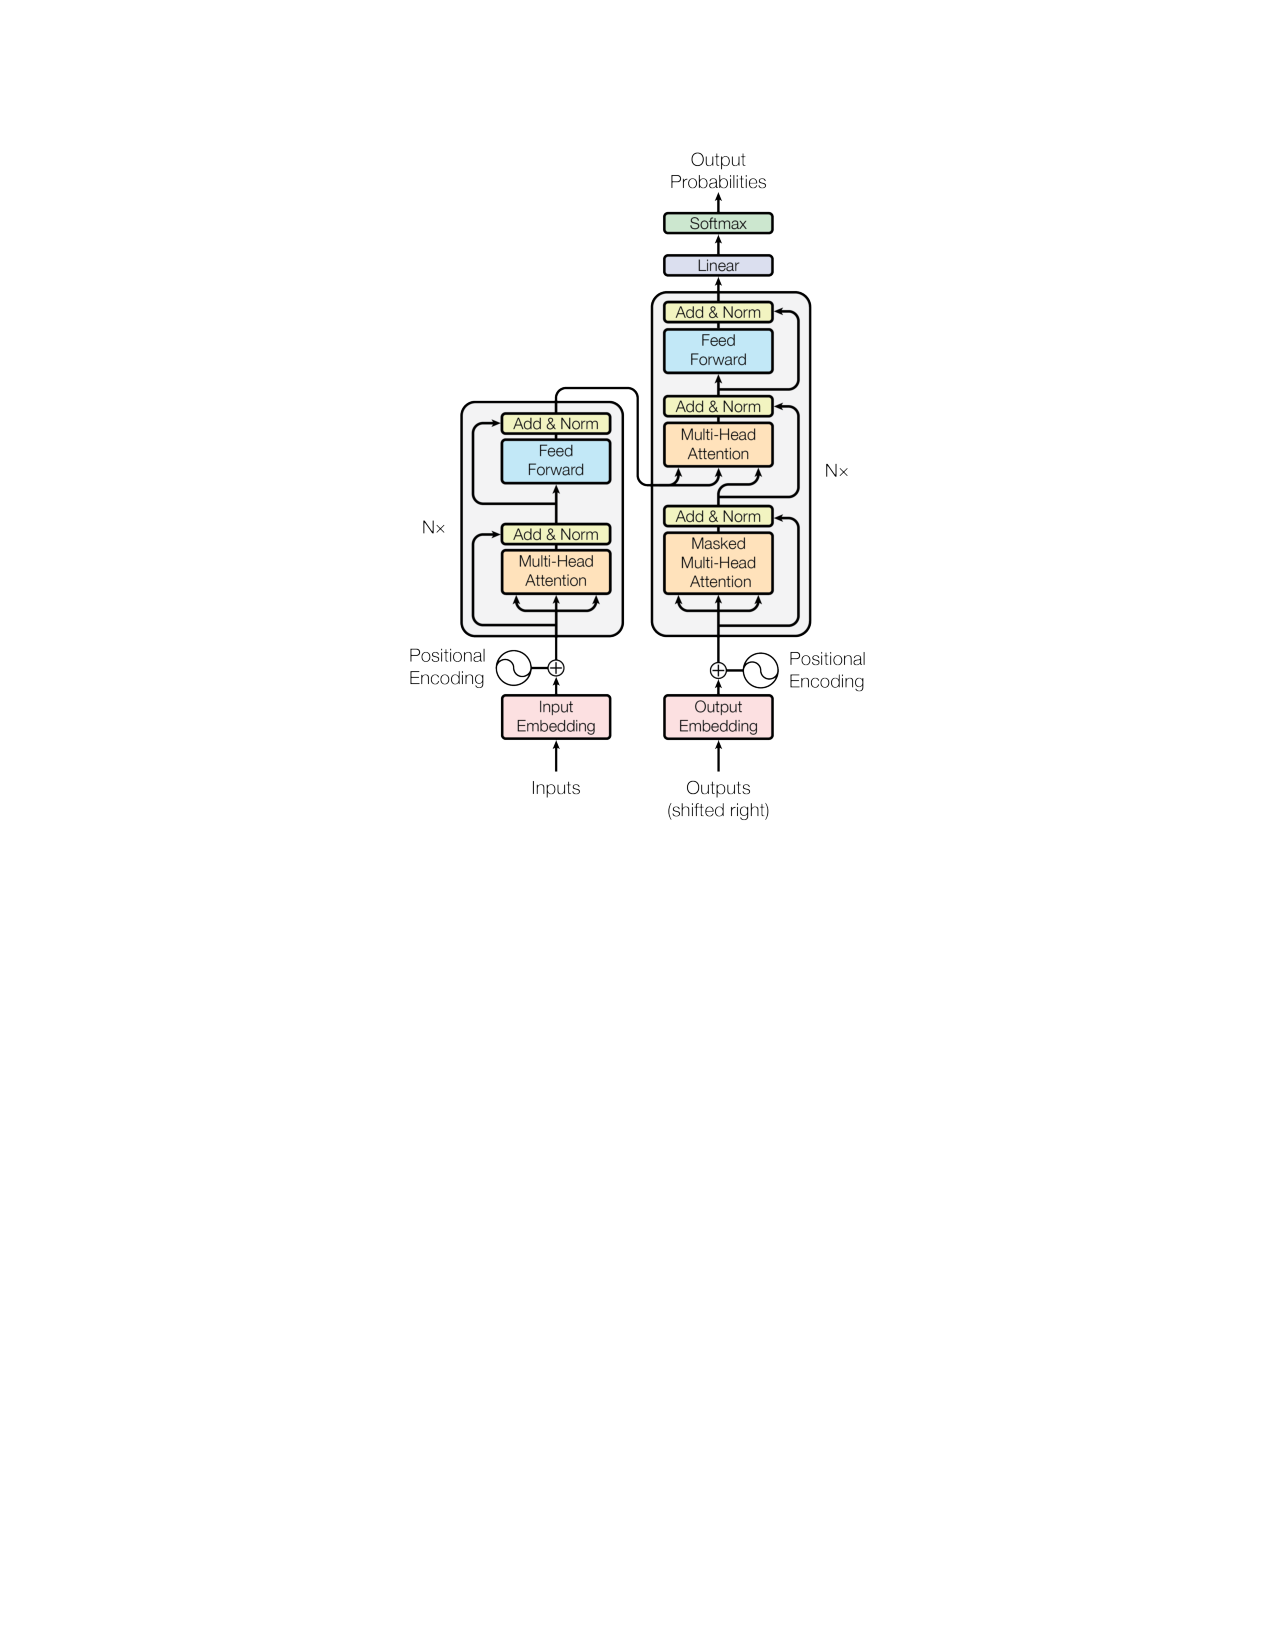
\includegraphics[width=10cm]{images/Transformer_architecture}}
        \caption[Figure of the transformer architecture.]{Transformer architecture proposed by Vaswani et al.\\
        Figure by Vaswani et al. \cite{vaswaniAttentionAllYou2017}.}
        \label{fig:transformer_architecture}
    \end{figure}


    
    %\subsection{Image Classification}


    %\subsection{Natural Language Processing}




% \section{Visual Question Answering}
    % What is VQA

    % Why is VQA important and interesting
    




\section{Model evaluation}
    In the field of machine learning and \gls{ai}, model evaluation refers to the process of measuring the quality and effectiveness of a trained model. These evaluations are essential in developing machine learning systems, allowing researchers and practitioners to determine their models' accuracy and generalization performance. Model evaluation helps to identify any weaknesses or shortcomings in a model's design or training process and enables researchers to make improvements to enhance the model's performance.

    \subsection*{Performance Metrics}
    \label{sec2:performance_metrics}
    Performance metrics are integral to machine learning models, allowing us to measure how well a model performs on a given task. These metrics evaluate the accuracy and effectiveness of a model's predictions by comparing them to the actual values. The choice of performance metrics depends on the problem being solved and the type of model being used. For example, in a binary classification problem, the model's accuracy can be used as a performance metric. In contrast, for multi-class classification problems, metrics like precision, recall, and $F_1$ score are more appropriate. In general, model evaluation metrics like precision and recall provide information about the performance of a model on a particular class, while accuracy and $F_1$ score provide an overall measure of model performance. Choosing appropriate performance metrics when developing a machine learning model is essential to ensure that the model's predictions align with the intended use case.
    
     % Precision and  Recall
    \subsection{Precision and Recall}
    Precision and recall are two important metrics used in classification tasks to evaluate the performance of a model. 
    Both precision and recall are based on the values in the confusion matrix, which is a table that summarizes the performance of a classification model. The confusion matrix contains four values: true positives, false positives, true negatives, and false negatives. True positives and false positives correspond to the model's positive predictions, while true negatives and false negatives correspond to the negative predictions. Figure \ref{fig:confusion_matrices} shows an example of a confusion matrix. The precision and recall are defined as follows.
        

    \begin{itemize}
        \item Precision: the ratio of correct answers among all answers proposed by the model, and it measures how precise the model's positive predictions are. The precision score can be calculated as follows:
        
        \begin{equation}
            \text{Precision} = \frac{\text{True Positive}}{\text{True Positive} + \text{False Positive}}
        \end{equation}
        
        \item Recall: the ratio of correct answers proposed by the model among all possible correct answers, and it measures how well the model is able to identify positive instances. The recall score can be calculated as follows:

        \begin{equation}
            \text{Recall} = \frac{\text{True Positive}}{\text{True Positive} + \text{False Negative}}
        \end{equation}
    \end{itemize}


    \begin{figure}[htb]
     \centerline{
         \begin{subfigure}[b]{0.5\textwidth}
             \centering
             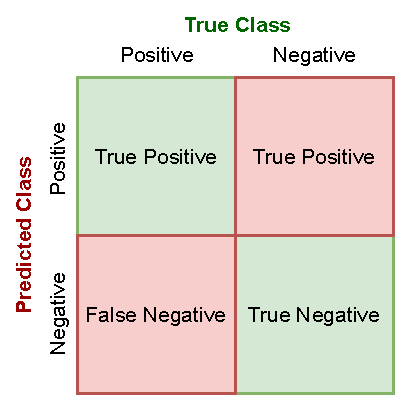
\includegraphics[width=\textwidth]{images/confusion_matrix_binary}
             \caption{Example of a confusion matrix of a binary classifier. A perfect classifier would have just true predictions.}
             \label{fig:confusion_binary}
         \end{subfigure}
         \hspace{0.1\textwidth}
         \begin{subfigure}[b]{0.5\textwidth}
             \centering
             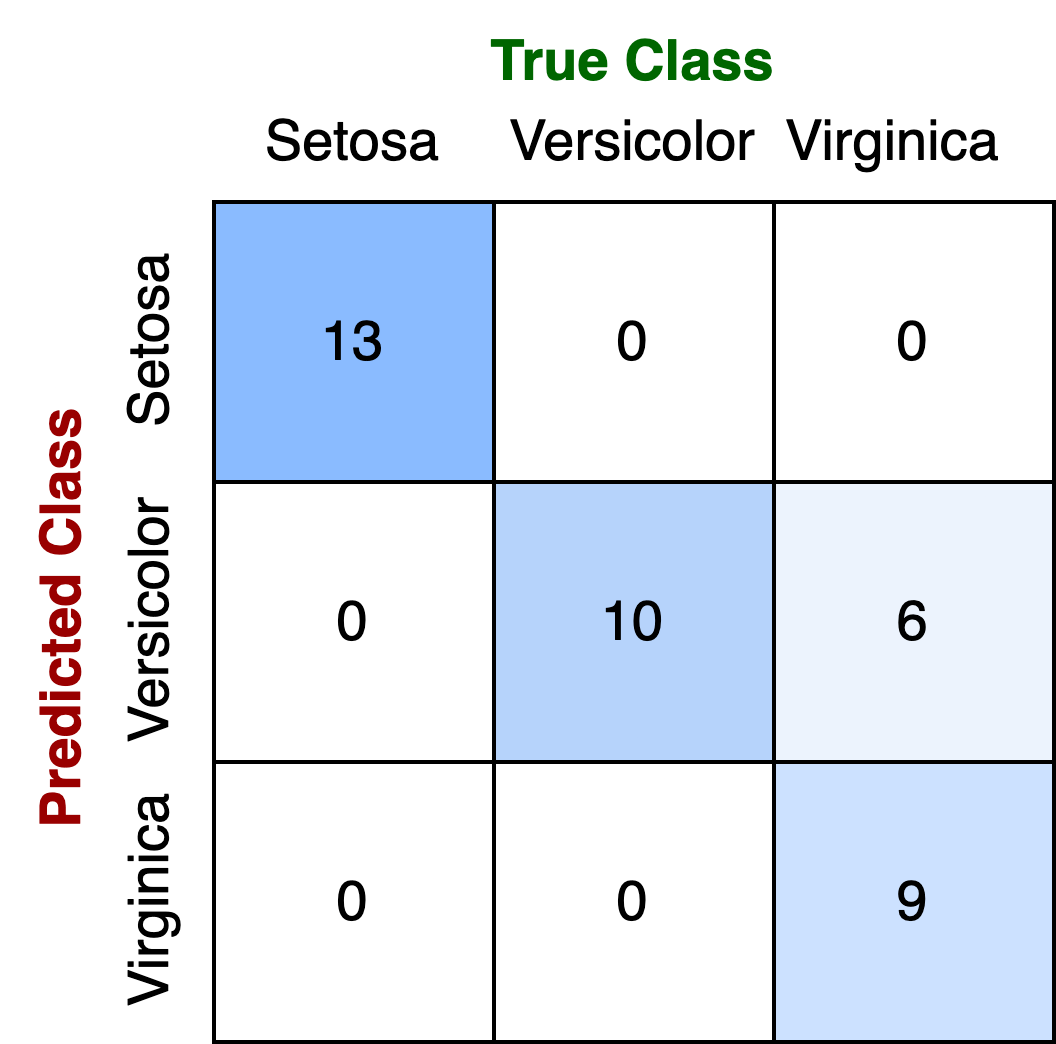
\includegraphics[width=\textwidth]{images/confusion_matrix_multi}
             \caption{Example of a confusion matrix of a multi-class classifier. An adapted example from scikit-learn \cite{ConfusionMatrix}.}
             \label{fig:confusion_multi}
         \end{subfigure}
         }
        \caption[Example of confusion matrices, both binary and multi-class.]{Example of confusion matrices, both for a binary (a) and multi-class (b) classifier.%Figure by the author.
        }
        \label{fig:confusion_matrices}
    \end{figure}


    % Accuracy
    \subsection{Accuracy}
\begin{comment}
https://www.statology.org/f1-score-vs-accuracy/
Accuracy:

Pro: Easy to interpret. If we say that a model is 90% accurate, we know that it correctly classified 90% of observations.

Con: Does not take into account how the data is distributed. For example, suppose 90% of all players do not get drafted into the NBA. If we have a model that simply predicts every player to not get drafted, the model would correctly predict the outcome for 90% of the players. This value seems high, but the model is actually unable to correctly predict any player who gets drafted.
\end{comment}
    Accuracy is a commonly used evaluation metric in statistics and artificial intelligence for classification models. It is a metric that is easy to interpret by humans because it measures the percentage of correctly predicted labels out of all the predictions made by the model. Accuracy is a valuable metric when the classes in the dataset are balanced, meaning that the number of instances for each class is roughly equal. However, when the classes are imbalanced, accuracy can be misleading. For instance, in a dataset with 95\% of the samples belonging to class A and only 5\% belonging to class B, a model that always predicts class A will have an accuracy of 95\% but will not be helpful in practice if the real-world data does not have the same distribution.

    Moreover, accuracy does not account for false positives and false negatives, as seen in Formula \ref{eq:accuracy}. False positives occur when the model predicts a positive label for a sample that is negative, while false negatives occur when the model predicts a negative label for a sample that is positive. In some applications, such as medical diagnosis, false negatives may be more costly than false positives, and accuracy alone may not be an adequate metric for evaluating model performance. Therefore accuracy can be a helpful and easily understandable metric when there is no critical downside predicting false negatives and the classes in the dataset are balanced. When dealing with real-world datasets, the classes are often not balanced, and a more suitable metric can be the $F_1$ score.
    


    \begin{equation}
        \text{Accuracy} = \frac{\text{True Positive} + \text{True Negative}}{\text{Total Sample Size}}
        \label{eq:accuracy}
    \end{equation}


    % F1 score
    \subsection{F\textsubscript{1} Score}


    The $F_1$ score is a statistical metric used to measure a model's performance on a dataset. It evaluates the performance of a binary classifier, which is a classification system that makes predictions for two possible classes, for example, positive and negative. The $F_1$ score can be calculated using the formula in Equation \ref{eq:f1}.

    \begin{equation}
        F_1 = 2 \frac{\text{Precision} \cdot \text{Recall}}{\text{Precision} + \text{Recall}}
        \label{eq:f1}
    \end{equation}

    In the context of question answering by an \gls{llm}, the $F_1$ score can be used to evaluate the accuracy of the model's responses to questions. Specifically, the score measures the harmonic mean of the model's precision and recall.

    \begin{comment}
https://www.statology.org/f1-score-vs-accuracy/
F1 Score:

Pro: Takes into account how the data is distributed. For example, if the data is highly imbalanced (e.g. 90% of all players do not get drafted and 10% do get drafted) then F1 score will provide a better assessment of model performance.

Con: Harder to interpret. The F1 score is a blend of the precision and recall of the model, which makes it a bit harder to interpret.

As a rule of thumb:

We often use accuracy when the classes are balanced and there is no major downside to predicting false negatives.

We often use F1 score when the classes are imbalanced and there is a serious downside to predicting false negatives.
    \end{comment}


    \subsection{Perplexity}

    Perplexity, often referred to as \textit{PPL}, is one of the most common metrics for evaluating language models. In information theory, perplexity measures how well a probability distribution or model predicts a sample. Intuitively, perplexity means being surprised, and in practice, it measures how surprised the model is when it sees new data. The lower the perplexity score, the better the training. Perplexity is usually only used to determine how well a model has learned the training set. 

    At its core, a language model is a probability distribution over a set of words, known as the model vocabulary. Considering all of its previous words, the model indicates the probability that a given word will appear in the vocabulary. Usually, the word with the maximum likelihood is selected as the next predicted word in the sequence.

    As an evaluation metric, perplexity can be used to compare probabilistic models, and low perplexity indicates that the probability distribution is good at predicting the sample. This probability can be calculated by multiplying a sequence of conditional probabilities for each word by its previous words, which indicates the probability of this sequence.
    Given a tokenized sequence $X = (x_0, x_1, ..., x_t)$, the perplexity of the sequence \textit{X} is given in the Formula \ref{eq:2_perplexity}.
        

    \begin{equation}
    \operatorname{Perplexity}(X)=\exp \left\{-\frac{1}{t} \sum_i^t \log p_\theta\left(x_i \mid x_{<i}\right)\right\}
    \label{eq:2_perplexity}
    \end{equation}

    In this formula, $\log p_\theta\left(x_i \mid x_{<i}\right)$ is the log-likelihood for the token with index $i$, given the previous tokens $x_{<i}$.

\section{Frameworks}
    %\subsection{PyTorch}
    This section briefly describes the most important external frameworks used in this thesis.
    
    \subsection{TensorFlow}
    
    TensorFlow is the framework used in the FLEX-VQA method proposed in this thesis. Here the framework is used to train the FLEX model to find connections between images and captions. A more detailed description of the implementation is discussed in Chapter \ref{sec:3_alpaca_vqa}.

    
    TensorFlow is an open-source machine learning framework developed and maintained by the Google Brain team. It was first introduced in 2015 and has since become one of the most widely used frameworks in machine learning.
    TensorFlow's core strength lies in its ability to handle large-scale machine learning models easily. It provides a highly optimized execution engine that efficiently computes complex models. This optimization is achieved through dataflow graphs, representing the computations as a directed graph of nodes and edges. Each node in the graph represents an operation, while the edges represent the data flow between operations. This architecture allows for parallelism and efficient computation, making it an attractive choice for large-scale machine learning tasks.
    
    One of the key advantages of TensorFlow is its versatility. It supports various machine learning tasks, including classification, regression, clustering, and reinforcement learning. It also supports deep learning models, such as \glspl{cnn}, \glspl{rnn}, and transformers.

    

    \subsection{Text Tokenization}
    \label{sec2:text_tokenization}

    Large language models such as GPT-3 \cite{brownLanguageModelsAre2020} and BERT \cite{devlinBERTPretrainingDeep2019} are trained on massive amounts of text data and can generate coherent and contextually relevant sentences, paragraphs, and even longer texts. However, feeding raw text data to such models can be computationally expensive and lead to suboptimal results due to high input variability. Therefore, text pre-processing techniques such as tokenization convert raw text into a form the model can more easily process.
    
    Tokenization is the process of splitting text into smaller units, called tokens, such as words, subwords, or characters. These tokens are then assigned a unique integer identifier and are often converted into fixed-length sequences, which can be fed into the language model. This process allows the model to handle text data more efficiently, reduces input variability, and helps to improve the training and inference times.
    
    Using a tokenizer specific to the language model used is crucial because it ensures that the tokens are consistent with the vocabulary and encoding scheme of the model. For example, using a tokenizer that splits words differently than the one used during the pre-training of the model can lead to inconsistencies and decreased performance.
    
    Various tokenization techniques are available, such as byte-pair encoding (BPE) \cite{gageNewAlgorithmData1994, sennrichNeuralMachineTranslation2016}, WordPiece \cite{devlinBERTPretrainingDeep2019}, and SentencePiece \cite{kudoSentencePieceSimpleLanguage2018}. BPE is a subword tokenization method that progressively merges the most frequent pairs of characters in a corpus to create a fixed-size vocabulary. WordPiece is a similar technique that uses a predefined list of subword units to tokenize words. SentencePiece is a more flexible method for creating a custom vocabulary that can handle rare and out-of-vocabulary words.
    
    Each of these techniques has its advantages and disadvantages. BPE and WordPiece are efficient and widely used, but they can result in a large vocabulary size and require additional processing steps to handle out-of-vocabulary words. SentencePiece can manage rare and out-of-vocabulary words better but can be computationally expensive due to their adaptive nature.

    This work uses a tokenizer built on top of SentencePiece, adapted and trained specifically to the \gls{llama} model. A more detailed explanation of this tokenizer can be seen later in \autoref{sec3:text_encoding}, which details the implemented method.
\label{sec:2_problem_and_application}
\section{Problem and application}
% Intro to this chapter

The increasing use of \gls{ai} has led to significant advances in various areas. However, understanding their decision-making processes becomes increasingly difficult as AI systems become more complex and opaque. 
The need for \gls{xai} and more transparent machine learning models has become imperative to address this problem, especially in applications where the consequences of wrong decisions can be severe, such as healthcare, finance, and autonomous vehicles. This chapter aims to provide an overview of the problem and application of \gls{xai}, which is crucial for building transparent and trustworthy \gls{ai} systems.


% Problem:
\subsection{Problem}
% ------------------------------------------

% Black-box
Although deep networks have made significant positive achievements in areas such as object detection \cite{girshickRichFeatureHierarchies2014, renFasterRCNNRealTime2015, redmonYouOnlyLook2016, linFocalLossDense2017}, image annotation and captioning \cite{vinyalsShowTellNeural2015, karpathyDeepVisualSemanticAlignments2015, johnsonDenseCapFullyConvolutional2016, tranRichImageCaptioning2016}, their complexity makes it more difficult to understand why these networks predict what they do. People, both researchers and users, of these systems need to be able to know how these black-box algorithms work to gain confidence \cite{koehlerExplanationImaginationConfidence1991, herlockerExplainingCollaborativeFiltering2000, dzindoletRoleTrustAutomation2003}, improve the models and apply these networks in new ways and domains \cite{jiangArtificialIntelligenceHealthcare2017, tonekaboniWhatCliniciansWant2019, holzingerCausabilityExplainabilityArtificial2019, guptaDeepLearningObject2021, tjoaSurveyExplainableArtificial2021}. Researchers and model architects can understand at a higher level how information flows in the network compared to everyday users by using their technical insight. However, as the architecture grows more profound and complex, and the training datasets are getting larger, it can be challenging to understand which parts of the input data contributed to making the decision \cite{sagirogluBigDataReview2013}.

% Interpretablity vs. accuracy 
\paragraph{Interpretablity vs. Accuracy\\}
The models with the highest accuracy for large data sets often have such complex architectures that even domain experts have difficulty interpreting their decisions \cite{caruanaIntelligibleModelsHealthCare2015}. Meanwhile, smaller, less complex architectures often have lower accuracy and generalize worse than their more complex counterparts. An example of this was shown in a case study to predict the risk of death for patients with pneumonia to help medical staff prioritize \cite{cooperPredictingDireOutcomes2005}. The researchers found the most accurate model to be a neural network, outperforming less complex models such as logistic regression. A rule-based system was also evaluated, and while this is a simpler model than neural networks, it is interpretable by design. This rule-based model to investigate the underlying dataset showed that a patient suffering from pneumonia and asthma had a lower probability of dying than only having pneumonia and was, therefore, less important to treat. The model drew this conclusion because patients in the training set with both pneumonia and asthma were usually prioritized first, was given medical treatment, and therefore had a higher survival rate \cite{cooperEvaluationMachinelearningMethods1997}. Because of this insight from the rule-based method, more complex models, such as neural networks, were concluded to be too risky in real-world decisions.

In pursuing models with higher accuracies, the primary way to achieve this is with even more complex models and larger training datasets \cite{bianchiniComplexityNeuralNetwork2014}. This brings the trade-off of an interpretable and explainable model vs. a more accurate model \cite{barredoarrietaExplainableArtificialIntelligence2020} to the forefront of discussion. 


% XAI
\paragraph{Explainable AI\\}
The field of \gls{xai} is working on solving the trade-off between performance and explainability. Some approaches specialize in explaining specific architectures, called model-specific. Meanwhile, others, called model-agnostic, try to explain models of different architectures, exploiting inherent properties in neural networks and statistics. Examples of inherently explainable models include decision trees, Bayesian classifiers, logistic regression, linear models, and \gls{knn} \cite{fixDiscriminatoryAnalysisNonparametric1989, coverNearestNeighborPattern1967, molnarInterpretableMachineLearning}. These algorithms are interpretable and, as a result of this, more explainable by design. This interpretability results from their internal structure, and computations follow clear rules or formulas that are manageable to comprehend.
However, models such as deep neural networks can work better than less complex methods on larger datasets. Because of their complex structure, with many hidden layers and weights trained on large datasets, it is difficult, if not impossible, for humans to understand what the model evaluated when choosing a prediction. Researchers in \gls{xai} have developed model-specific and \textit{post-hoc} model-agnostic techniques to understand better these complex methods to explain the underlying model prediction. The term post-hoc comes from Latin and means \textit{"after this"}. In this thesis, the term is used to describe a method applied after a machine learning model is developed. These methods try to bridge the gap between high accuracies and explainability.
In theory, this allows us to use the model best fit for the task, regardless of complexity, without the expense of not understanding the model's predictions. 

% Many models 
Different explanations try to give additional insights into the predictions. A local explanation looks at one specific model decision and tries to explain what was important in the input data to provide this prediction. A global explanation, on the other hand, looks at the whole model's process of making decisions and sees how the different attributes contribute to making a decision. These global explanations can also be built from multiple local faithful explanations. A third type is contrastive explanations that utilize local features to explain the difference between instances. This allows insight into the model's inner workings on a more global scale based on local predictions.

% Cons
One typical disadvantage of model-agnostic explanations is that their insights and descriptions are not always faithful to the underlying model they try to explain. This can happen if an explaining model is trained to look at the underlying model's input, inner workings, and output and learns the correlation between them. The problem is that correlation does not imply causation, and the explaining model can give a deceiving explanation that can look correct at first. Developing explanatory methods that find causations rather than correlations is an ongoing research topic.




% Application (where my system will go):
\subsection{Application}
% ------------------------------------------

% Intro
With better explanations that are intuitive and faithful to the underlying prediction model, humans can be more precise when improving the model. This also gives the ability to use the model with confidence that the prediction is based on correct decisions.


% Medical / bank
When machine learning methods are utilized as a tool in the real world, it is essential that everyone in the process of using the tool can trust the model. 
In a medical setting, both the doctor and the patient must have confidence that the conclusions drawn are based on a reasonable and trustworthy basis. If the model is correct, but the clinician does not trust the underlying model or the patient has no explanation for the model's conclusion, the model is not being used as intended and is, therefore, a useless tool.

This is also the case in other domains, such as finance. Here the bank can utilize large models that look at the loan applicant using big data. The bank can profile the customer alongside fellow citizens in the same demographic and use a model to predict whether or not that customer should receive a loan. In this case, finding all biases in the data set can be difficult, as it can be challenging to distinguish correlation from causation in demographic analysis \cite{garciaHarmsDemographicBias2019}. Here the bank must have an explanation alongside the predicted output of the loan to see better if the model made a trustworthy decision. 

% Non-experts improve models



% Finding bias in datasets
One advantage of better understanding the model's evaluations in a prediction is that it can highlight biases in the dataset. If these biases are known and understood, they can be combated. Ribeiro et al. \cite{ribeiroWhyShouldTrust2016} showed that it could be hard to discover biases when the predictions are correct without knowing the reasoning. They experimented with a model trained on images of huskies and wolfs and first presented the model's prediction without explanations to participants. The participants were then asked to determine if they trusted the model. Thereafter the model's explanation for the predictions was presented, and participants again had to tell if they trusted the model now. In both instances, the participants were also asked if they thought snow was a potential feature of importance. An image of a husky misclassified as a wolf can be seen in Figure \ref{fig:wolf_husky}, alongside the regions important in making the decision. The results can be seen in Table \ref{table:husky_vs_wolf}, and it can be seen that a considerable amount of the participants lost trust in the biased model when they were presented with the explanation. They then noticed that the decision was based only on whether the snow was visible in the image. This shows that models with an intuitive explanation are more likely to gain the trust of their users. Trustworthy explanations open the ability for users who do not have insight into the making of the model to still able to detect biases in the dataset and improve the model. 

\begin{table}[htb]
    \centering
    \begin{tabular}{ c c c} 
     
               & Before explanation & After explanation\\ [0.5ex] 
        \Xhline{1.5pt} \\ 
            Trusted the biased model & 10 out of 27 & 3 out of 27 \\  [0.5ex]
        \hline  \\ 
            Thought snow was an \\ important feature & 12 out of 27 & 25 out of 27 \\ [1ex] 
        \hline
    \end{tabular}
    \caption[Overview over the trust by participants in the "Husky vs. Wolf" experiment by Ribeiro et al. \cite{ribeiroWhyShouldTrust2016}.]{Overview over the trust by participants in the "Husky vs. Wolf" experiment by Ribeiro et al. \cite{ribeiroWhyShouldTrust2016}. The majority lost trust when explained that a classifier considered snow in the background the most important feature when classifying images of huskies and wolves.}
    \label{table:husky_vs_wolf}
\end{table}

\begin{figure}[htb]
    \centering
    \includegraphics[width=\linewidth]{images/husky_vs_wolf.png}
    \caption[Husky classified as a wolf, alongside an explanation of what the model considered important.]{Husky classified as a wolf, alongside an explanation of what the model considered important.\\ Figure by Ribeiro et al. \cite{ribeiroWhyShouldTrust2016}.}
    \label{fig:wolf_husky}
\end{figure} 


% Make humans able to learn from the models
Today's machine learning models are already better than humans in domain-specific tasks, like chess \cite{campbellDeepBlue2002}. Silver et al. \cite{silverGeneralReinforcementLearning2018} proposed the reinforcement learning algorithm AlphaZero, which learns to play chess, shogi (Japanese chess), and Go, only by playing with itself. This method does not get any domain knowledge except the game rules and achieves performance better than humans. Because this algorithm has not seen humans play these games, it does not have human biases and playing flaws in it, and professional game players can learn new moves and techniques by playing with it. 
As performance better than humans is a goal many researchers strive for when it comes to machine learning, it is more important than ever that these algorithms give explanations on what they do and why so that humans can learn new aspects never before thought of, as well as detect flaws that restrict performance, both in humans and machines.

\label{sec:2_related_work}
\section{Related Work} 

% Computer vision
% ------------------------------------------
\subsection{Computer Vision}
Computer Vision is the interdisciplinary task of making computers understand and act on visual input. This scientific discipline's main objective is to make computers extract high-dimensional data from the real world using digital images and videos. The extraction of visual information that computers can use includes methods for collecting, processing, analyzing, and understanding the images using statistics, geometry, physics, and learning theory. 

% Object detection
Object detection is a significant part of computer vision that has made astonishing progress. It has been an important research topic because it is one of the fundamental problems in computer vision. Detecting objects form the fundamental basis of other computer vision tasks, such as object tracking, segmentation, and image captioning. Many of these sub-domains' achievements have come from using \gls{cnn} architectures with more layers, trained on larger datasets, and more powerful computers. These main components have made the algorithms capable of learning a deeper understanding of the visual world and learning more fundamental elements of materials, objects, and scenes.  

% Is this relevant?
Krizhevsky et al. introduced AlexNet\cite{krizhevskyImageNetClassificationDeep2017}, as a variant of the \gls{cnn} proposed by LeCun et al.\cite{lecunHandwrittenDigitRecognition1989, lecunGradientbasedLearningApplied1998} seen in Figure \ref{fig:lenet}, both utilizing the backpropagation algorithm \cite{rumelhartLearningRepresentationsBackpropagating1986}
in training. The main difference is that AlexNet uses three more layers, ReLu \cite{fukushimaCognitronSelforganizingMultilayered1975}
, and is running on \glspl{gpu} instead of \glspl{cpu}, which in practice means more efficient use of computing power.
AlexNet achieved impressive results in the ImageNet \cite{dengImageNetLargeScaleHierarchical2009} 2012 Challenge and is often considered the most influential paper published in computer vision. 
Following this paper, there has been an increasing amount of work done and articles published in the domain of deep learning and images during the last decade.

\begin{figure}[htb]
    \centerline{
    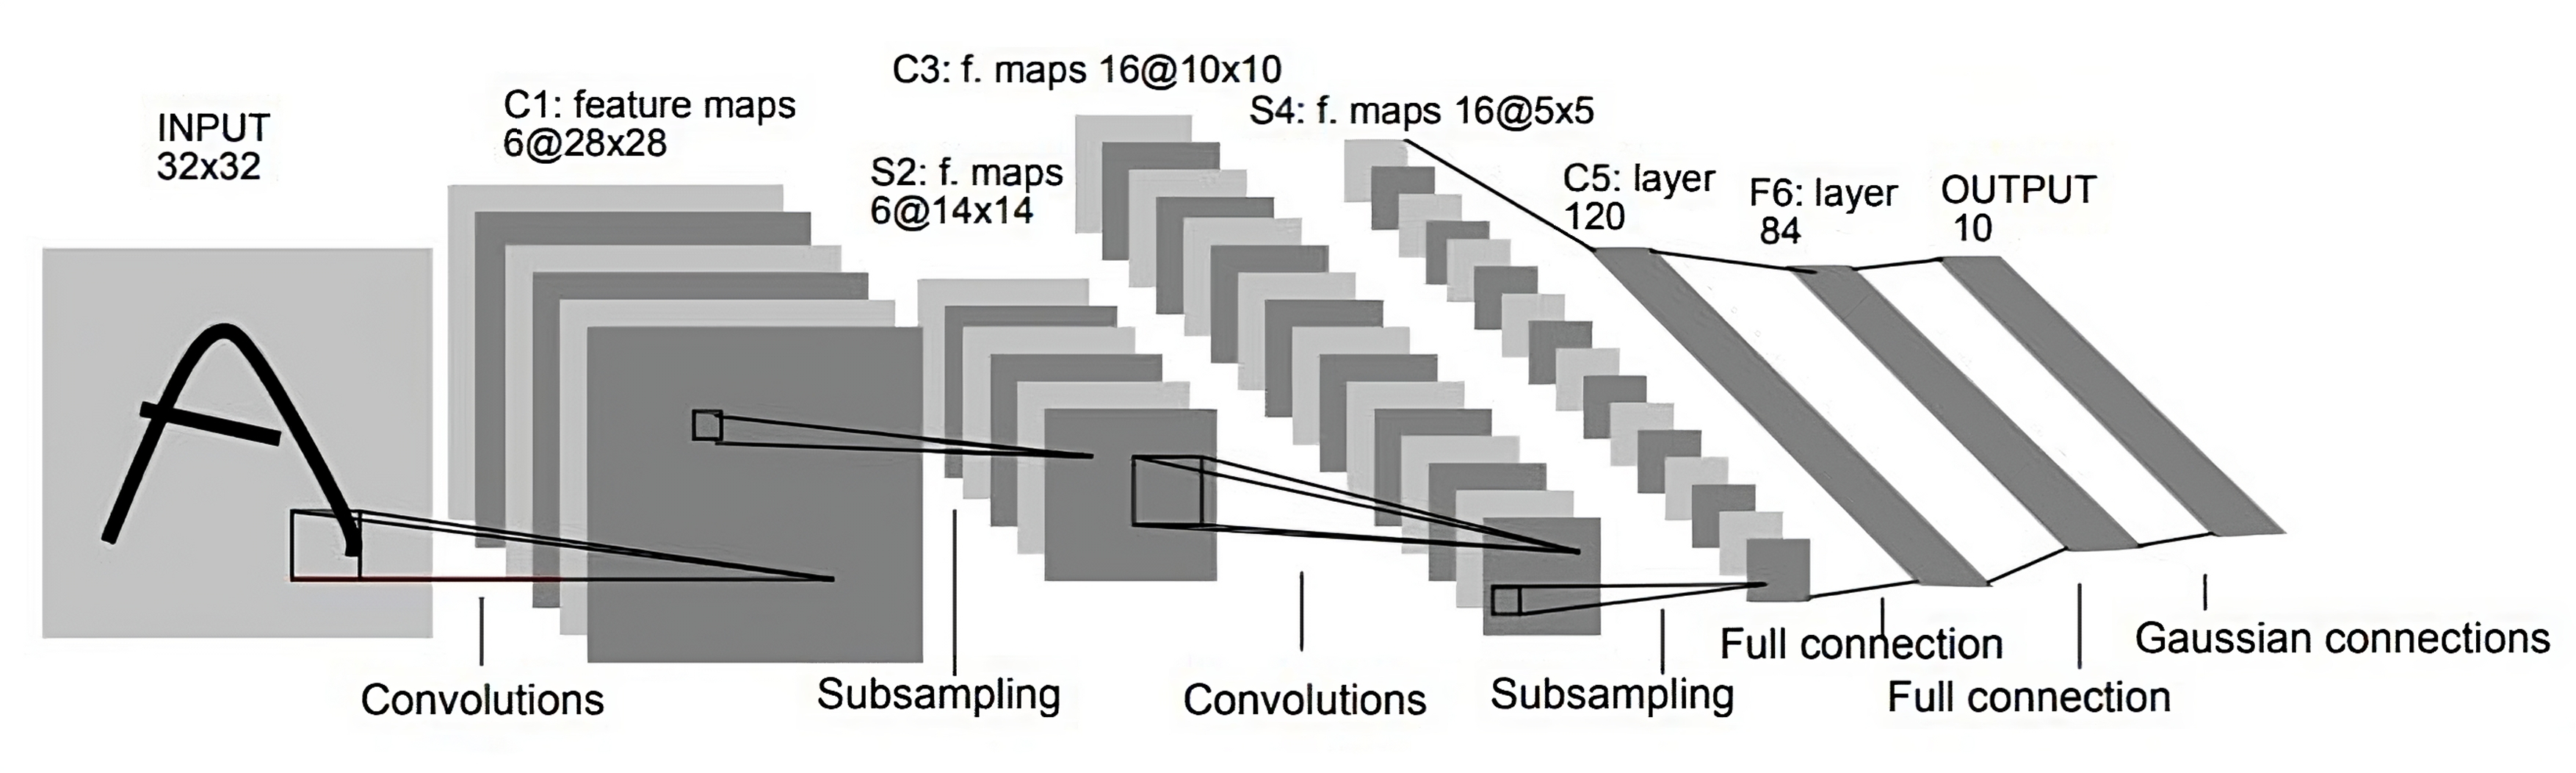
\includegraphics[width=1.2\linewidth]{images/LeNet.jpeg}}
    \caption{\gls{cnn} architecture of LeNet-5 proposed by LeCun et al. \cite{lecunGradientbasedLearningApplied1998}.}
    \label{fig:lenet}
\end{figure} 

% XAI
% ------------------------------------------
\subsection{Explainable AI (XAI)}

The rapid growth of artificial intelligence (AI) technologies has led to an increasing demand for transparency and interpretability in machine learning models. While these models have demonstrated impressive performance in various applications, their lack of transparency and interpretability has raised concerns about their reliability, accountability, and potential biases. As a result, the field of explainable AI (XAI) has emerged to address these challenges by developing techniques and tools that enable humans to understand how AI systems work and make decisions.

Explainable AI is an interdisciplinary research field that aims to make AI models more transparent, interpretable, and accountable to human users. It combines techniques from machine learning, human-computer interaction, cognitive science, and other related disciplines to develop methods and tools for explaining the behavior and decisions of AI models. The need for explainable AI arises from the fact that many machine learning models, especially deep neural networks, are often viewed as black boxes, meaning that their internal workings and decision-making processes are intricate for humans to comprehend. As a result, these models' lack of transparency and interpretability can create distrust among users, limit their adoption, and raise ethical concerns, especially in high-stakes applications such as healthcare, finance, and criminal justice.

An overview of influential methods proposed in \gls{xai} is presented in this subsection.

% LIME
\paragraph{LIME\\}
In pursuing a method that helps the explaining model to be locally faithful to the underlying model, Ribeiro et al. \cite{ribeiroWhyShouldTrust2016} proposed \gls{lime}. This model-agnostic method explains any method by learning an interpretable, less complex model locally around a specific prediction. This approach assures that the explanation is locally accurate and represents the actual inner workings of the model. 
In the same paper, they also introduce a method for explaining the global attributes of the model by framing the task as a submodular optimization problem. The technique is called SP-LIME (Submodular Pick LIME). With this approach, they can achieve global explanations that are locally accurate and faithful to the underlying model in a non-redundant way. LIME will be used later in this thesis as an explanation method adapted to a \gls{llm}.

% SHAP
\paragraph{SHAP\\}
Making non-redundant explanation features faithfully and efficiently is not easy. Lundberg et al. \cite{lundbergUnifiedApproachInterpreting2017} proposed a unified framework for interpreting predictions made by the underlying method. This framework called \gls{shap}, assigns each feature a value of importance for a specific prediction. The framework utilizes the class of additive feature attribution methods and estimates the Shapley % cite
values from cooperative game theory for that prediction. With this approach, they achieve more effective explanations to compute and have better consistency with human intuition than previously proposed methods.  


% Grad-CAM
\paragraph{Grad-CAM\\}
Visually explaining features that contributed to an image prediction can be essential in gaining trust in a model. Selvaraju et al. \cite{selvarajuGradCAMVisualExplanations2020} proposed a technique for making \glspl{cnn} more explainable and transparent by producing visual explanations for the underlying model. The method is called \gls{gradcam}, a generalization of CAM proposed by Zhou et al. \cite{zhouLearningDeepFeatures2016}, and uses the gradients in a single backtrack of any target concept. Therefore it does not need any architectural changes or retraining of the underlying prediction model to produce a localization map highlighting the crucial regions in the image for predicting the given concept, often called a saliency map in computer vision.

% DenseCap


% FLEX
\paragraph{FLEX\\}
While visual-only explanations can give the user insight into which areas of the image were essential in making the decision, they tell little to nothing about why those regions were important. On the other hand, linguistic descriptions give the user an essential understanding of the model's evaluation when predicting. 
Wickramanayake et al. \cite{wickramanayakeFLEXFaithfulLinguistic2019} propose \gls{flex} to merge saliency maps with locally accurate linguistic descriptions. In this approach, they look at the gradients through layers and identify the most critical activations in the single decision. The advantage of looking at different layers is that alongside getting an explanation that is faithful to the underlying model, they also extract features the \gls{cnn} identifies at each layer. A \gls{cnn} may represent high-level concepts, like a "car", at the last layer while identifying features such as texture and color at earlier layers. Using the activations at all essential layers, \gls{lime} achieves an image caption that explains all the essential parts of the prediction using sentences. \gls{flex} maps words to neurons in the \gls{cnn} by looking at high activations of that neuron combined with a word from the caption during the training. For this, they are using a \gls{cnn} and two stacked \gls{lstm} \cite{hochreiterLongShorttermMemory1997} cells.
The \gls{flex} framework is used as a basis for one of the two proposed methods in this thesis. A more detailed description of the specific implementation for this work is discussed later in Chapter \ref{sec3:flex_vqa}.

% VQA dataset
\paragraph{Visual Question and Answering (VQA)\\}
In order to make the linguistic abilities of computers more robust, Agrawal et al. \cite{agrawalVQAVisualQuestion2016} proposed a new dataset called \gls{vqa}. This dataset provides images from the COCO dataset \cite{linMicrosoftCOCOCommon2015}, paired with free-form, open-ended questions and answers corresponding to the content of the images. These questions and answers target different areas of the images, including underlying context and background details. This dataset aims to make models that can learn multi-modal visual and linguistic domain knowledge to get a more general and complete understanding of the world. Models that have done well in this dataset are frequently made up of \glspl{cnn}, to acquire the visual knowledge, combined with an \gls{rnn} % cite
for linguistic understanding.

Even though \gls{vqa} is not strictly \gls{xai}, it is still relevant regarding transparency to the user. \gls{vqa} is an important research area because it provides AI systems with human-readable explanations of their decision-making processes.
By providing a natural language explanation of why a specific answer was generated for a particular question about an image, \gls{vqa} models can help improve \gls{ai} systems' transparency and interpretability. This can be particularly important in domains such as healthcare and finance, where trust and transparency are critical for ensuring that \gls{ai} systems are making reliable and safe decisions. Therefore, it is important to continue developing and improving \gls{vqa} models to provide accurate and interpretable answers to questions regarding images.
Both the methods implemented and investigated in this work will be based on \gls{vqa}, using text to describe the contents of images utilizing different approaches.

\subsection{Large Language Models (LLMs)}

    \glspl{llm} are neural networks with billions or more parameters trained by self-supervised or semi-supervised learning on large amounts of text. They originated around 2018 and have performed competently on a variety of tasks. \glspl{llm} are typically general-purpose models that excel in various roles, with their performance and range of capabilities depending on the number of resources devoted during training. These models demonstrate considerable general knowledge about the world and can learn associations that make the model "memorize" numerous facts and contexts during training. 

    
    
    \glspl{llm} are pre-trained on large text datasets and can be characterized by four parameters: the size of the model, the size of the training dataset, the training cost, and the post-training performance. These variables are related by simple statistical laws called scaling laws. 

    \glspl{llm} serve not only to teach \glspl{ai} human languages but to understand proteins, write software code, and help students. These models are trained with vast amounts of text fed into the AI algorithm through unsupervised learning, allowing the model to find valuable connections in the language. Through this method, a \gls{llm} learns words, their relationships, and the concepts behind them. Large language models can also be tailored for specific use cases, including through techniques such as fine-tuning or prompt tuning, which feed the model small bits of data that must be focused on to train it for a specific application.
    
    
    However, a disadvantage of \glspl{llm} is that they can suffer from a phenomenon called hallucinations. Generative models can hallucinate because they contain vast amounts of data and organize the information in an unsupervised way. These models tend to make self-confident claims about facts not justified by their training data, which appears plausible but is not factually correct. Because of their size, they can also be challenging and computationally expensive to interpret. An ethical concern about the size of these models is that they are also computationally intensive during training and inference since they are trained on large datasets. As a result, these models have a larger carbon footprint than smaller models. However, there are ways to make these models smaller and faster, which are discussed in this chapter and also provide an overview of the development of large language models.

   

    \paragraph{BERT\\}

    BERT (Bidirectional Encoder Representations from Transformers) is a large-scale neural language model that has made significant contributions to the field of natural language processing (NLP) \cite{devlinBERTPretrainingDeep2019}. BERT is a pre-trained model that uses a transformer-based architecture that has grown in popularity in recent years due to its success in several NLP tasks. Introduced by Google in 2018, BERT is trained on a large corpus of text using an unsupervised learning approach. The model is pre-trained on a task called Masked Language Modeling (MLM), in which a small percentage of the words in a sentence are masked randomly, and the model is trained to predict the original word based on the context of the sentence. This method can be viewed as a "fill in the blanks" task, often called a cloze test, of the training sentences, keeping some words invisible to the model during training and helping the model generalize to new and unseen data. In addition, BERT is trained on an NSP task (Next Sentence Prediction), similar to the GPT models. The model is given pairs of sentences and asked to predict whether the second sentence continues the first.

    The main innovation of BERT is its ability to understand the context and provide contextualized word embeddings. Unlike previous word embeddings, which were static and did not change based on the context of the sentence, BERT can offer different embeddings to the same word depending on its context.
    
    
    
    \paragraph{BART\\}
    Lewis et al. at Facebook presented an \glspl{llm} named BART (Bidirectional and Auto-Regressive Transformer) \cite{lewisBARTDenoisingSequencetoSequence2019}. Like BERT, it uses a transformer-based architecture and is trained on a large corpus of natural language. However, unlike BERT, BART is unique because it integrates a bidirectional and auto-regressive architecture, which makes it well-suited for text generation and summarization tasks. 
    This model is a pre-trained sequence-to-sequence model that can be fine-tuned for various natural language processing tasks. BART is designed to handle auto-regressive, non-auto-regressive, generation, and comprehension tasks. The model is pre-trained on a large corpus of text using a denoising autoencoder objective, which requires the model to reconstruct original text from corrupted versions. Using a denoising autoencoder in pre-training helps reduce hallucinations by training the model to distinguish between real and fake input. 
    The authors demonstrate that BART outperforms several state-of-the-art models on various natural language generation and comprehension tasks, including summarization, question answering, and text classification. They also show that BART can be fine-tuned with relatively little data and can generalize to new domains. 
    However, instead of using Masked Language Modeling and Next Sentence Prediction like BERT, BART is pre-trained using a denoising autoencoder (DAE) objective.

    The DAE objective involves corrupting an input sequence by randomly deleting or swapping tokens and training the model to reconstruct the original sequence. This approach allows BART to handle more complex tasks such as text summarization, sentence generation, and machine translation.
        
    
    
    \paragraph{GPT\\}
    GPT (Generative Pre-trained Transformer) is a set of \glspl{llm} developed by OpenAI \cite{radfordImprovingLanguageUnderstanding2018}. Like BERT and BART, GPT is a transformer-based model but uses only an autoregressive architecture. It is pre-trained on large datasets and tuned for specific tasks. When GPT-2 was released, it was trained on a much larger dataset with significantly more parameters than GPT-1 \cite{radfordLanguageModelsAre2019}. This allowed it to generate more coherent and realistic text than its predecessor. GPT-3 is the third model in the GPT series and was released by OpenAI in 2020. It was trained on an even larger dataset than GPT-2 and had even more parameters, making it one of the largest language models. GPT-3 could generate even more readable and human-like text than its predecessors and perform various NLP tasks without explicit training \cite{brownLanguageModelsAre2020}. At the time of writing, the last published GPT model was GPT-4, which is still an autoregressive model but also includes multimodality \cite{openaiGPT4TechnicalReport2023} by making it able to interpret images. To reduce the effects of hallucinations on a generated output, GPT implements a combination of methods such as filtering and sampling.
    
    These models have proven to be versatile and powerful tools for natural language processing. GPT models have significantly influenced the NLP field, and many researchers and developers have used it as a starting point for their projects. Fine-tuned chatbot versions of GPT-3 and GPT-4 have been made available for public interaction under the name ChatGPT \cite{ChatGPT}.

    
    
    
    
    % LLaMA
    \paragraph{LLaMA\\}
    The \gls{ai} department of Meta, previously Facebook, released a modified architecture for a \gls{llm} called \gls{llama} \cite{touvronLLaMAOpenEfficient2023}.
    %This model with corresponding weights was not released to the public, but after a leak, \cite{vincentMetaPowerfulAI2023}, both the model and its weights became available to the public. 
    These models are created to compare to other \glspl{llm}, such as GPT-3 \cite{brownLanguageModelsAre2020}, Chinchilla \cite{hoffmannTrainingComputeOptimalLarge2022}, or PaLM \cite{chowdheryPaLMScalingLanguage2022}, while keeping the number of parameters considerably smaller. In the paper where Hoffman et al. propose the Chinchilla model, they also present insight into how models scale the best in conjunction with the size of the available dataset. The authors of \gls{llama} use this insight to make the model with fewer parameters perform well by training it on more tokens. The dataset that the \gls{llama} model is pre-trained on is publicly available and disclosed, which makes it compatible with open-source. The architecture is based on the transformer \cite{vaswaniAttentionAllYou2017}, with various improvements inspired by other \glspl{llm}. Some of these improvements are pre-normalization, inspired by GPT-3 \cite{brownLanguageModelsAre2020}, which improves the training stability by normalizing the input of each transformer sub-layer instead of the output. Like the PaLM model, they also use a SwiGLU as the activation function, first introduced by Shazeer at Google \cite{shazeerGLUVariantsImprove2020}, instead of ReLU. Shazeer showed it to improve the perplexities of transformer-based models. To make the self-attention mechanisms in the transformer position-agnostic, the authors implement a method called Rotary Position Embedding (RoPE) introduced by Su et al. This method allows both flexibilities of sequence length and faster convergence in fine-tuning compared to normal self-attention. With the 13 billion parameter version of \gls{llama}, the authors show that this model outperforms the GPT-3, with 175 billion parameters, on several evaluation metrics. Because the \gls{llama} model is ten times smaller than GPT-3, it can also be run on a single \gls{gpu}. These steps towards smaller, capable models benefit both the carbon footprint and inference compute budget and permit democratizing \glspl{llm} by making a model that can run on consumer hardware.

    \paragraph{Alpaca\\}
    The work in this thesis uses this Alpaca model to interpret images. More of how this model is implemented is discussed later in Chapter \ref{sec3:alpaca_vqa}.
    
    With Taori et al., Stanford University released an open-source fork of this \gls{llama} model, with some modifications, called Alpaca \cite{taoriStanfordCRFM, taoriStanfordAlpacaInstructionfollowing2023}. The Alpaca model is a fine-tuned model, with a 7B \gls{llama} model as the base model, trained on 52 thousand instruction-following tasks generated by OpenAI's text-DaVinci-003 model \cite{OpenAIAPI} using techniques from the Self-Instruct paper proposed by Wang et al. \cite{wangSelfInstructAligningLanguage2022}. Figure \ref{fig:alpaca_training} shows an overview of the Alpaca training procedure and how the dataset was built. By using text-DaVinci-003 to generate instructions, the team was able to train the model and generate the dataset for a significant cost reduction compared to traditional methods, totaling only \$600, with \$500 using OpenAI API to create the dataset and \$100 to rent 3 hours on 8 Nvidia 80GB A100 GPU cards. Reducing the cost of training an \gls{llm}, comparable to models much more expensive to develop, helps democratize these models and make them available to more people for less cost and energy.

    
    To address the ethical issue of not knowing whether a text is generated by an \gls{ai}, the team also implemented the method proposed by Kirchenbauer et al. \cite{kirchenbauerWatermarkLargeLanguage2023}. This method embeds "green" or marked tokens into the generated text, which are invisible to humans but can be detected by an algorithm analyzing a short span of these tokens.  
    The authors argue that the watermark can be embedded with negligible impact on text quality and can be detected with an efficient open-source algorithm without access to the language model API or parameters. The watermark works by choosing a random set of green tokens before generating a word and using a soft watermarking rule to encourage the input of green tokens during sampling. The authors propose a statistical test to detect the watermark with interpretable p-values and derive an information-theoretic framework to analyze the sensitivity of the watermark.

    Given the need for less computational resources, giving the method a reduced carbon footprint, and the ability to disclose the generated text as computer-generated, the Alpaca model represents a favorably ethical and transparent option for users of a system compared to other \gls{llm}. As such, it is an appropriate choice as a starting point for this thesis. This model has many of the benefits that \glspl{llm} can provide, like knowledge of vasts amount of data, while still being able to customize it to a specific task through fine-tuning. This process enables the model to adapt to a particular assignment while retaining the knowledge acquired from its initial training data.

    
    % Data flow
    \begin{figure}[htb]
        \centerline{
        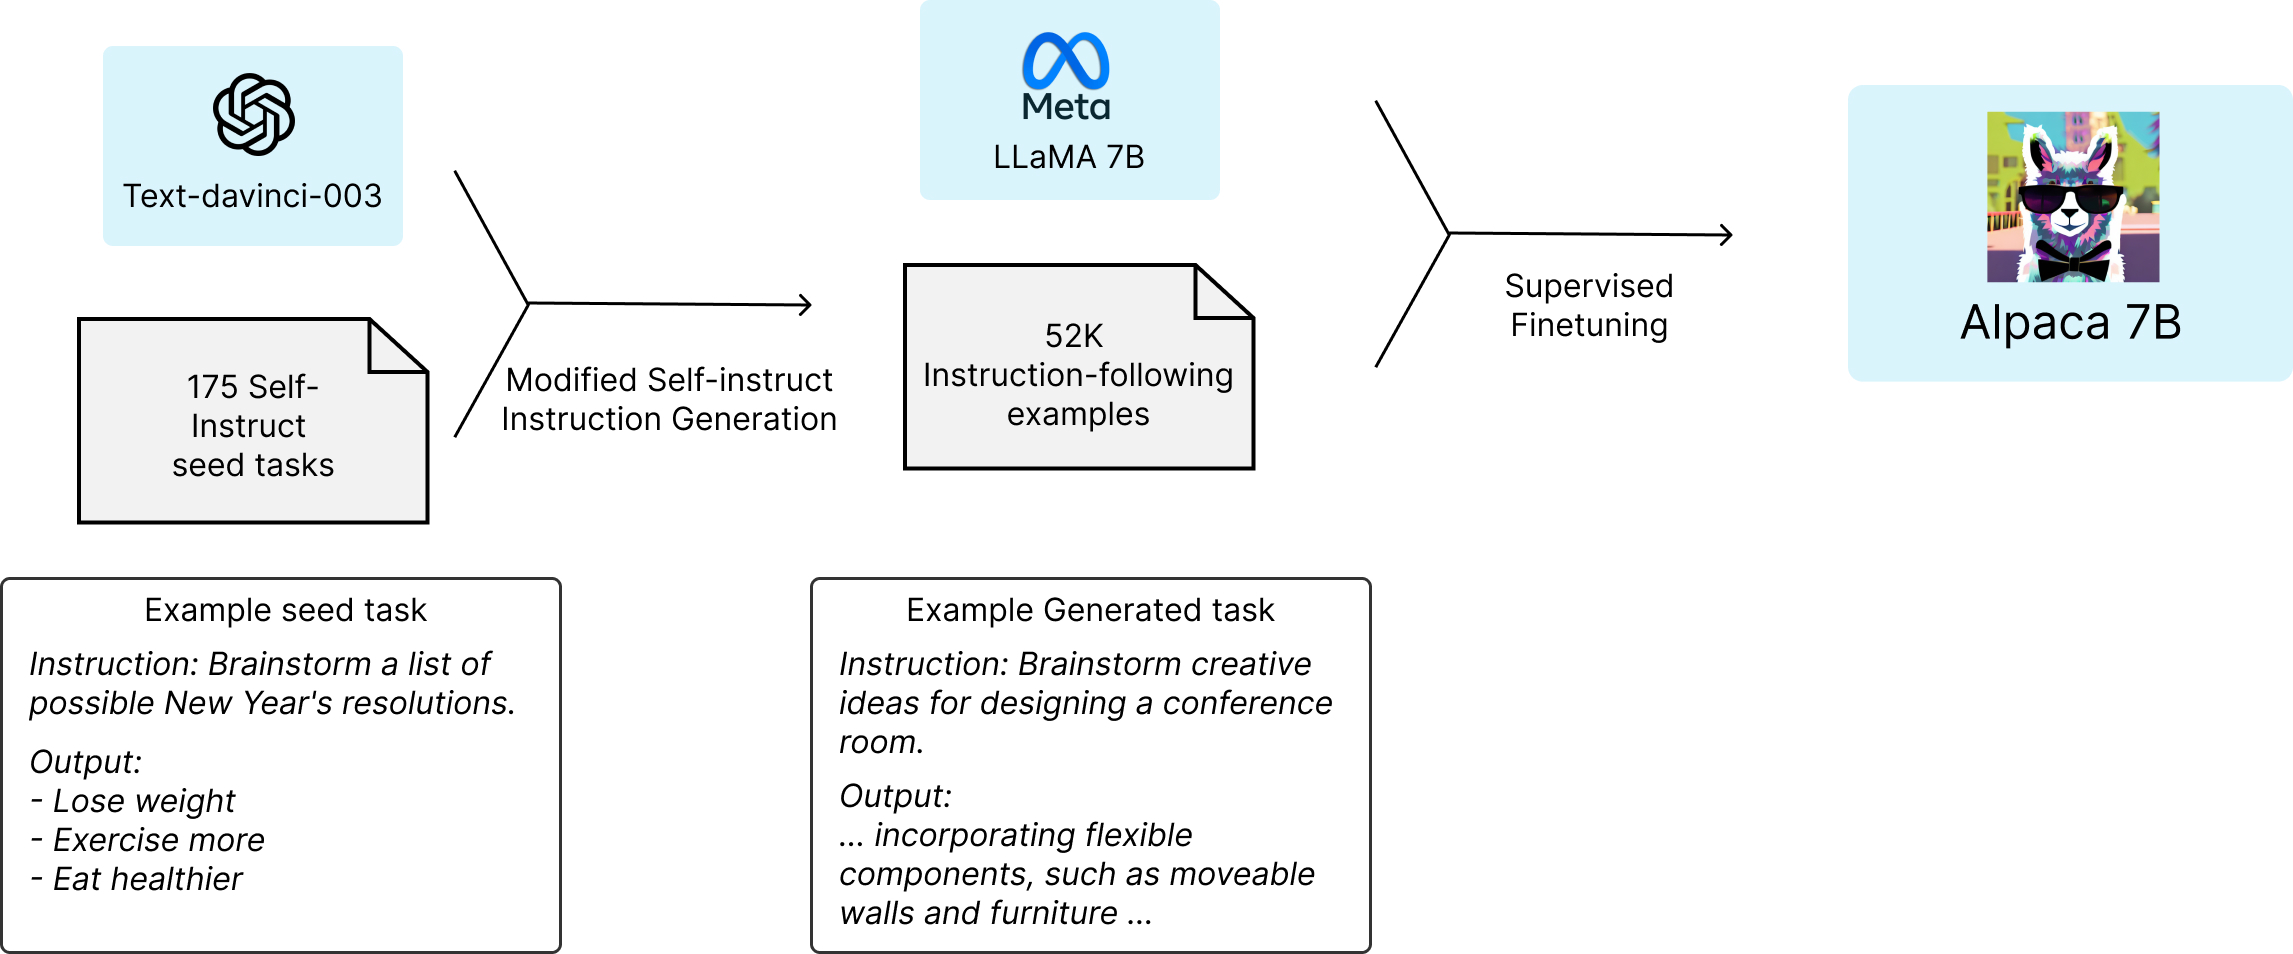
\includegraphics[width=17cm]{images/alpaca_framework.jpeg}}
        \caption[Overview of the Stanford Alpaca training procedure.]{Overview of the Stanford Alpaca training procedure.\\Figure credits: Taori et al. \cite{taoriStanfordCRFM}}
        \label{fig:alpaca_training}
    \end{figure}
\section{Summary}
\label{sec:2_summary}

\begin{comment}
SUMMARY: Often, we recommend ending this chapter (and all chapters after except the conclusion) with a summary section. The aim is to give an overview of, and tea-spoon-feeding the reader with, what he/she should have learned reading this chapter. What can be concluded from this chapter? How does the information given here give
 
arguments for your problem statement? Finally, lead to the next chapter (“... and we will therefore in the next chapter address these challenges, and describe our ideas/implementation/...”)
\end{comment}

\backmatter{}

\newpage
\printbibliography
\end{document}
